\documentclass[a4paper, 12pt]{report}
% Forces PDF version 1.7
\pdfminorversion=7
% Allows writing the document in french
\usepackage[utf8]{inputenc}
\usepackage[francais]{babel}
% Allows to use images
\usepackage{graphicx}
% Provides hyperlinks within the document
\usepackage{enumitem}
% Adds space between paragraphs
\usepackage{parskip}
% Supports Text Companion fonts (necessary for gensymb)
\usepackage{textcomp}
\usepackage{array}
\usepackage{multicol}
% Better tabular
\usepackage{tabularx}
% Allows to use colors
\usepackage{xcolor}
\usepackage[margin=4cm]{geometry}
\usepackage{varwidth}
% Euro
\usepackage{eurosym}
\usepackage{amsmath}
% Lipsum
\usepackage{lipsum}
\usepackage{listings}
\usepackage{color}

\definecolor{mygreen}{rgb}{0,0.6,0}
\definecolor{mygray}{rgb}{0.47,0.47,0.33}
\definecolor{myorange}{rgb}{0.8,0.4,0}
\definecolor{mywhite}{rgb}{0.98,0.98,0.98}
\definecolor{myblue}{rgb}{0.01,0.61,0.98}

\lstset{ %
  backgroundcolor=\color{mywhite},
  basicstyle=\footnotesize,
  breakatwhitespace=false,
  breaklines=true,
  captionpos=b,
  commentstyle=\color{mygray},
  deletekeywords={...},
  escapeinside={\%*}{*)},
  extendedchars=true,
  frame=shadowbox,
  keepspaces=true,
  keywordstyle=\color{myorange},
  language=Octave,
  morekeywords={*,...},
  numbers=left,
  numbersep=5pt,
  numberstyle=\tiny\color{mygray},
  rulecolor=\color{black},
  rulesepcolor=\color{myblue},
  showspaces=false,
  showstringspaces=false,
  showtabs=false,
  stepnumber=2,
  stringstyle=\color{myorange},
  tabsize=2,
  title=\lstname
}
\usepackage{float}

\setcounter{secnumdepth}{5}

\usepackage[
    type={CC},
    modifier={by-nc-nd},
    version={4.0},
]{doclicense}

\usepackage[colorlinks=true,urlcolor=black,linkcolor=black]{hyperref}
% New columns types
% Left
\newcolumntype{L}{>{\raggedright\arraybackslash}X}
% Center
\newcolumntype{C}{>{\centering\arraybackslash}X}
% Right
\newcolumntype{R}{>{\raggedleft\arraybackslash}X}

% Add more space before and after table
\newenvironment{centerspace}{\setlength{\topsep}{1ex}\center}{\endcenter}
% Sets the color of gray.
\newcommand{\gray}{\rowcolor[gray]{.90}}
% Allows to draw lines.
\newcommand{\HRule}{\rule{\linewidth}{0.5mm}}
% Uses the arabic numerals for sections.
\renewcommand{\thesection}{\arabic{section}}

% Width of text.
\addtolength{\textwidth}{2cm}
% Odd page left margin.
\addtolength{\oddsidemargin}{-1cm}
% Height of main text.
\addtolength{\textheight}{2cm}
% Removes indentation.
\setlength\parindent{0pt}
% Indicates overflow words.
\setlength{\overfullrule}{10pt}
% Height of items.
\setitemize{itemsep=1em}

% Starts roman numbering (trick to not numbering the first pages)
\pagenumbering{roman}

\begin{document}
\renewcommand{\bibname}{Références}
\begin{center}
  
\includegraphics[scale=0.12]{textures/logo/heh.pdf}

  \vspace{1cm}

  \textsc{\LARGE Laboratoire d'Arduino : Rapport} \\ [1cm]

  \textsc{\large 1\up{er} Bachelier en Informatique} \\ [0.2cm]

  \begingroup
  \fontfamily{pag} \selectfont

  \HRule \\ [0.4cm] {
    \huge Electricité et élément d'électronique pour l'interfaçage informatique \\ [0.2cm]
  }
  \HRule \\ [1.3cm]
  \endgroup

  \begin{minipage}[t]{0.4 \textwidth}
    \begin{flushleft}
      \large \emph{Auteur:} \\
	  Timothée \textsc{Simon}
    \end{flushleft}
  \end{minipage}
  %
  \begin{minipage}[t]{0.4 \textwidth}
    \begin{flushright}
      \large \emph{Enseignant :} \\
	  David \textsc{Arnaud}
    \end{flushright}
  \end{minipage}

  \vspace{2.5cm}

  
\includegraphics[scale=0.08]{textures/logo/technical.pdf}

  \vspace{0.5cm}

  Année académique 2016 - 2017
\end{center}

\thispagestyle{empty}
\clearpage
\newpage
\thispagestyle{empty}
\setcounter{page}{0}
\null
\newpage
\clearpage
\mbox{~}
\vfill
Ce document est mis à disposition selon les termes de la licence Creative
Commons “\href{https://creativecommons.org/licenses/by-nc-nd/4.0/}{Attribution
- Pas d'utilisation commerciale 4.0 International}”.

\begin{center}
  
\includegraphics[scale=1]
    {textures/images/license/license.pdf}
\end{center}
\setcounter{page}{0}
\thispagestyle{empty}

\newpage
\pagenumbering{arabic}
\tableofcontents
\newpage
\chapter{Introduction}
Dans ce rapport nous allons utiliser un Arduino Uno ainsi que toute une série de modules compris dans un coffret. Arduino est une plateforme de développement open source via des cartes de développement. Puisque le projet est open source, les schemas des cartes est disponnible gratuitement ainsi que la suite logicielle Arduino que nous avons utilisé dans ces manipulations.
L'Arduino que nous utilisons est l'Arduino Uno qui possède 14 entrés/sortie numérique dont 6 sont compatibles PWM et 6 entrées/sorties analogiques. Il possède également une prise USB pour injecter notre code ou pour l'alimenter et une prise d'alimentation jack. Efin, un bouton reset est présent pour `rebooter' l'Arduino.
\begin{figure}[h]
	\centering
	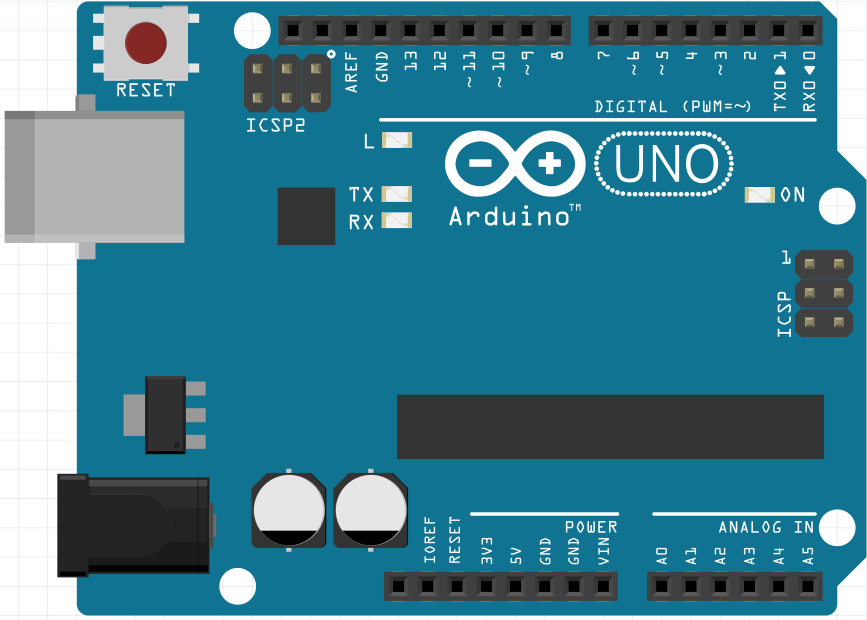
\includegraphics[height=3cm]{img/arduino.png}
	\caption{\label{ArduinoBoard}Arduino Board}
\end{figure}
Pour la programation de l'Arduino nous utillisons la suite officielle d'Arduino disponible gratuitement. Pour les schematiques nous avons utilisé Fritzing, également fournis gratuitement par la fondation Arduino.
\begin{figure}[h]
	\centering
	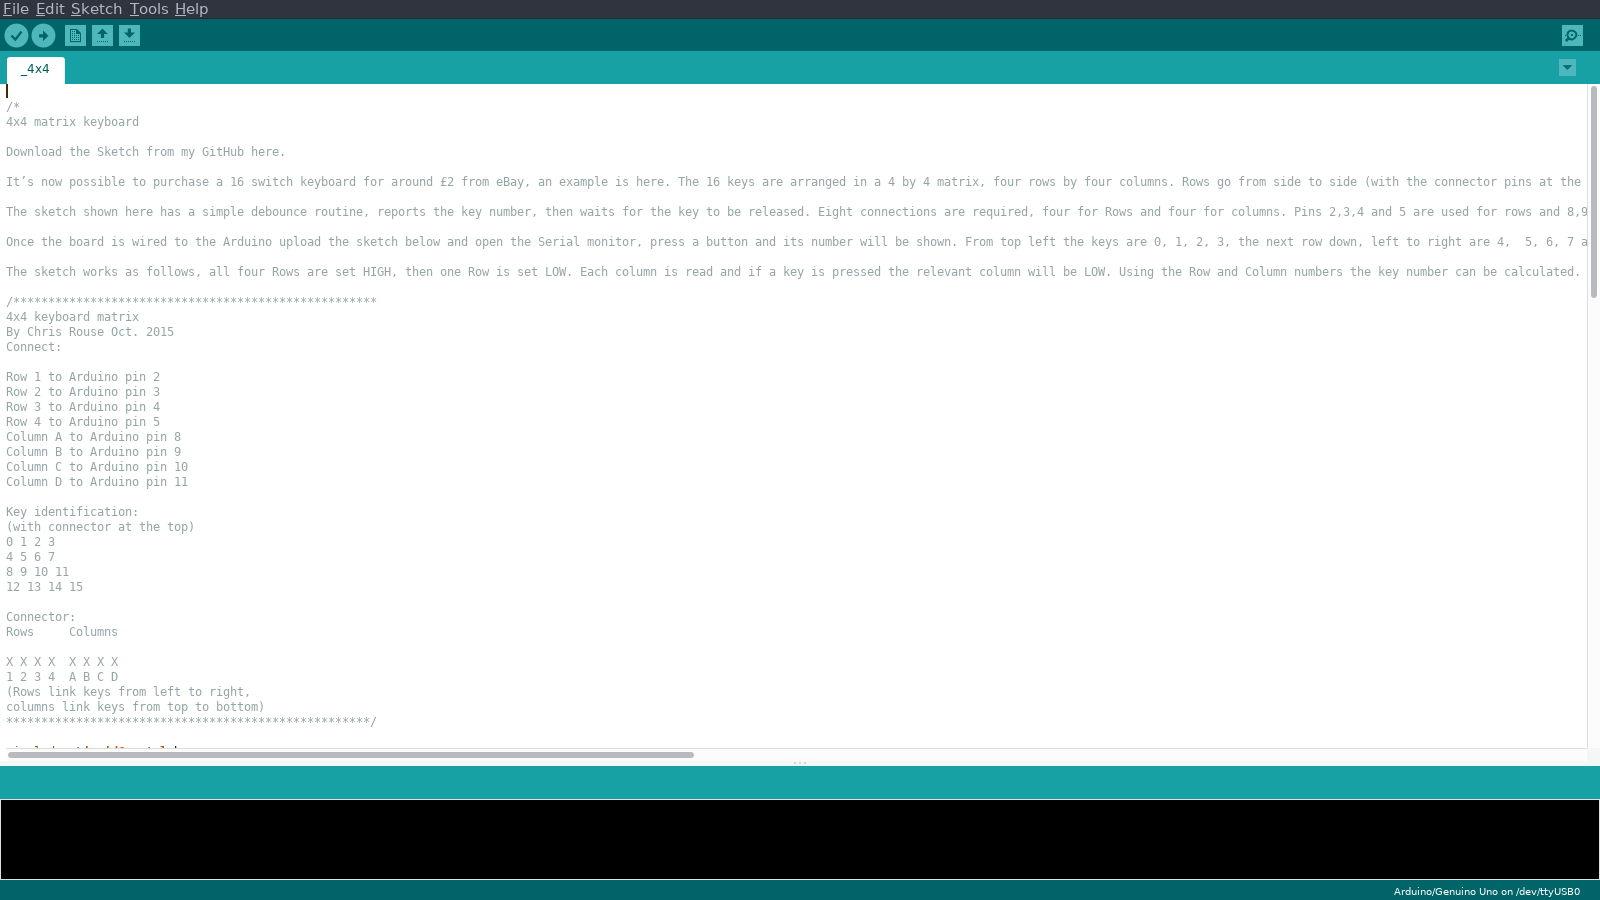
\includegraphics[height=6cm]{img/suite.png}
	\caption{\label{SuiteArduino}Suite Arduino}
\end{figure}
\begin{figure}[h]
	\centering
	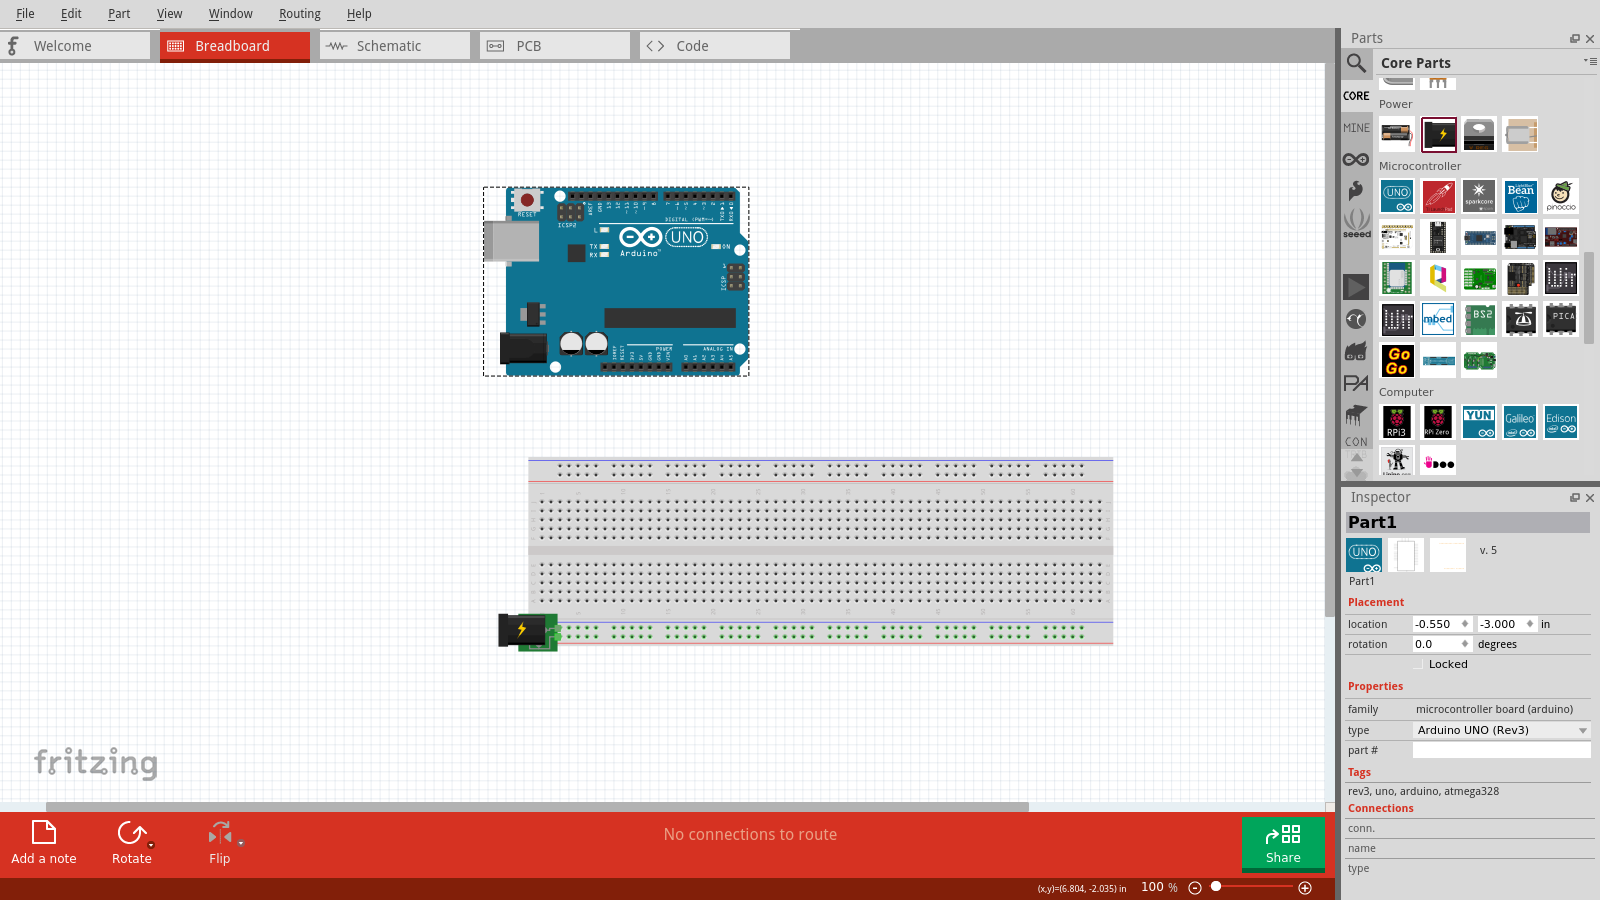
\includegraphics[height=6cm]{img/fritzing.png}
	\caption{\label{Fritzing}Fritzing}
\end{figure}
\clearpage
\chapter{Manipulations}
\section{TP1: Bling Bling}
\subsection{Objectif}
Dans ce TP nous allons commencer par faire clignoter une LED, puis nous utilserons la led RGB poru afficher une couleur précise, finalement nous ferons un compte à rebour avec l'afficheur 7 segments et l'afficheur 4 fois 7 segments.

\subsection{Matériel}
\begin{itemize}
	\item Un ordinateur
	\item Un arduino Uno R3
	\item Une LED simple
	\item Une LED RGB
	\item Un afficheur 7 segments
	\item Un afficheur 4 fois 7 segments
	\item Une résistance de 220$\Omega$
\end{itemize}

\subsection{LED clignotante}
Dans cette manipulation nous allons faire clignotter une LED en la branchant au port 13 de l'arduino. Ce port correspond également à la LED inclue dans l'arduino, nous pourrions donc même ici nous passer de la breadboard. Nous mettons bien sur aussi une résistance de 220$\Omega$ en série avec la LED, mais nous aurions aussi pu utiliser la résistance \textit{pullup}.
\lstinputlisting[language=C]{Code/TP1/TP1.1/TP1.1.ino}
\begin{figure}[H]
	\centering
	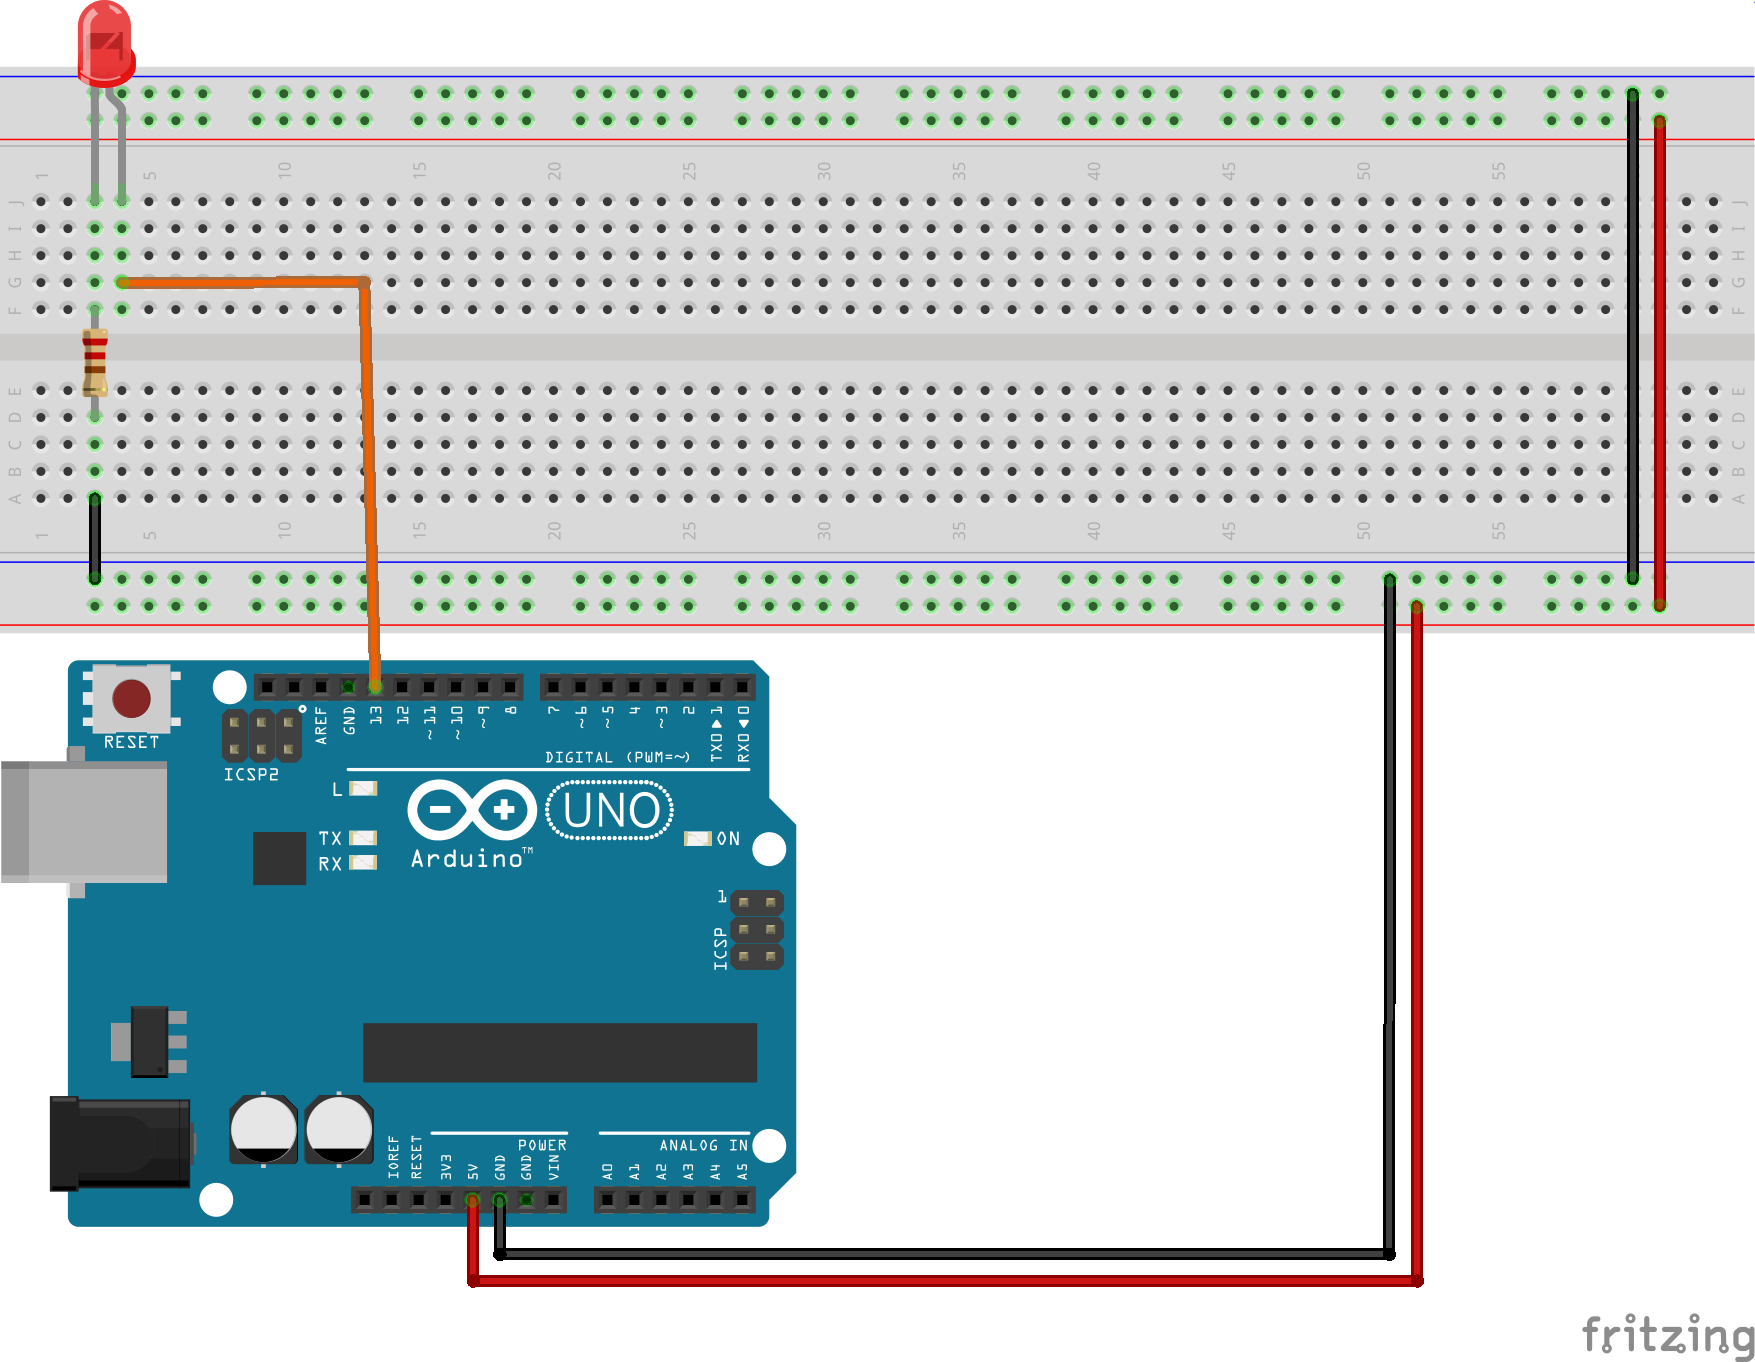
\includegraphics[height=6cm]{img/TP1-1.png}
	\caption{\label{TP1.1}LED clignotante}
\end{figure}
%TODO LED

\subsection{LED RGB}
Dans cette manipulaton nous allons controller la couleur d'une LED RGB qui est en faite composée de 3 LED, une rouge, une verte et une bleu. Nous relions donc les pattes correspondantes aux couleurs à notre arduino et la patte correspondant à la cathode commune au +VCC via une résistance\@. Le code correspondant à une LED RGB à annode commune est aussi inclu. Nous utilisons les ports analogiques et non digitaux pour pouvoir controler l'intensité de chaque couleur et ainsi allumer la LED de la couleur souhaitée.
\lstinputlisting[language=C]{Code/TP1/TP1.2/TP1.2.ino}
\begin{figure}[H]
	\centering
	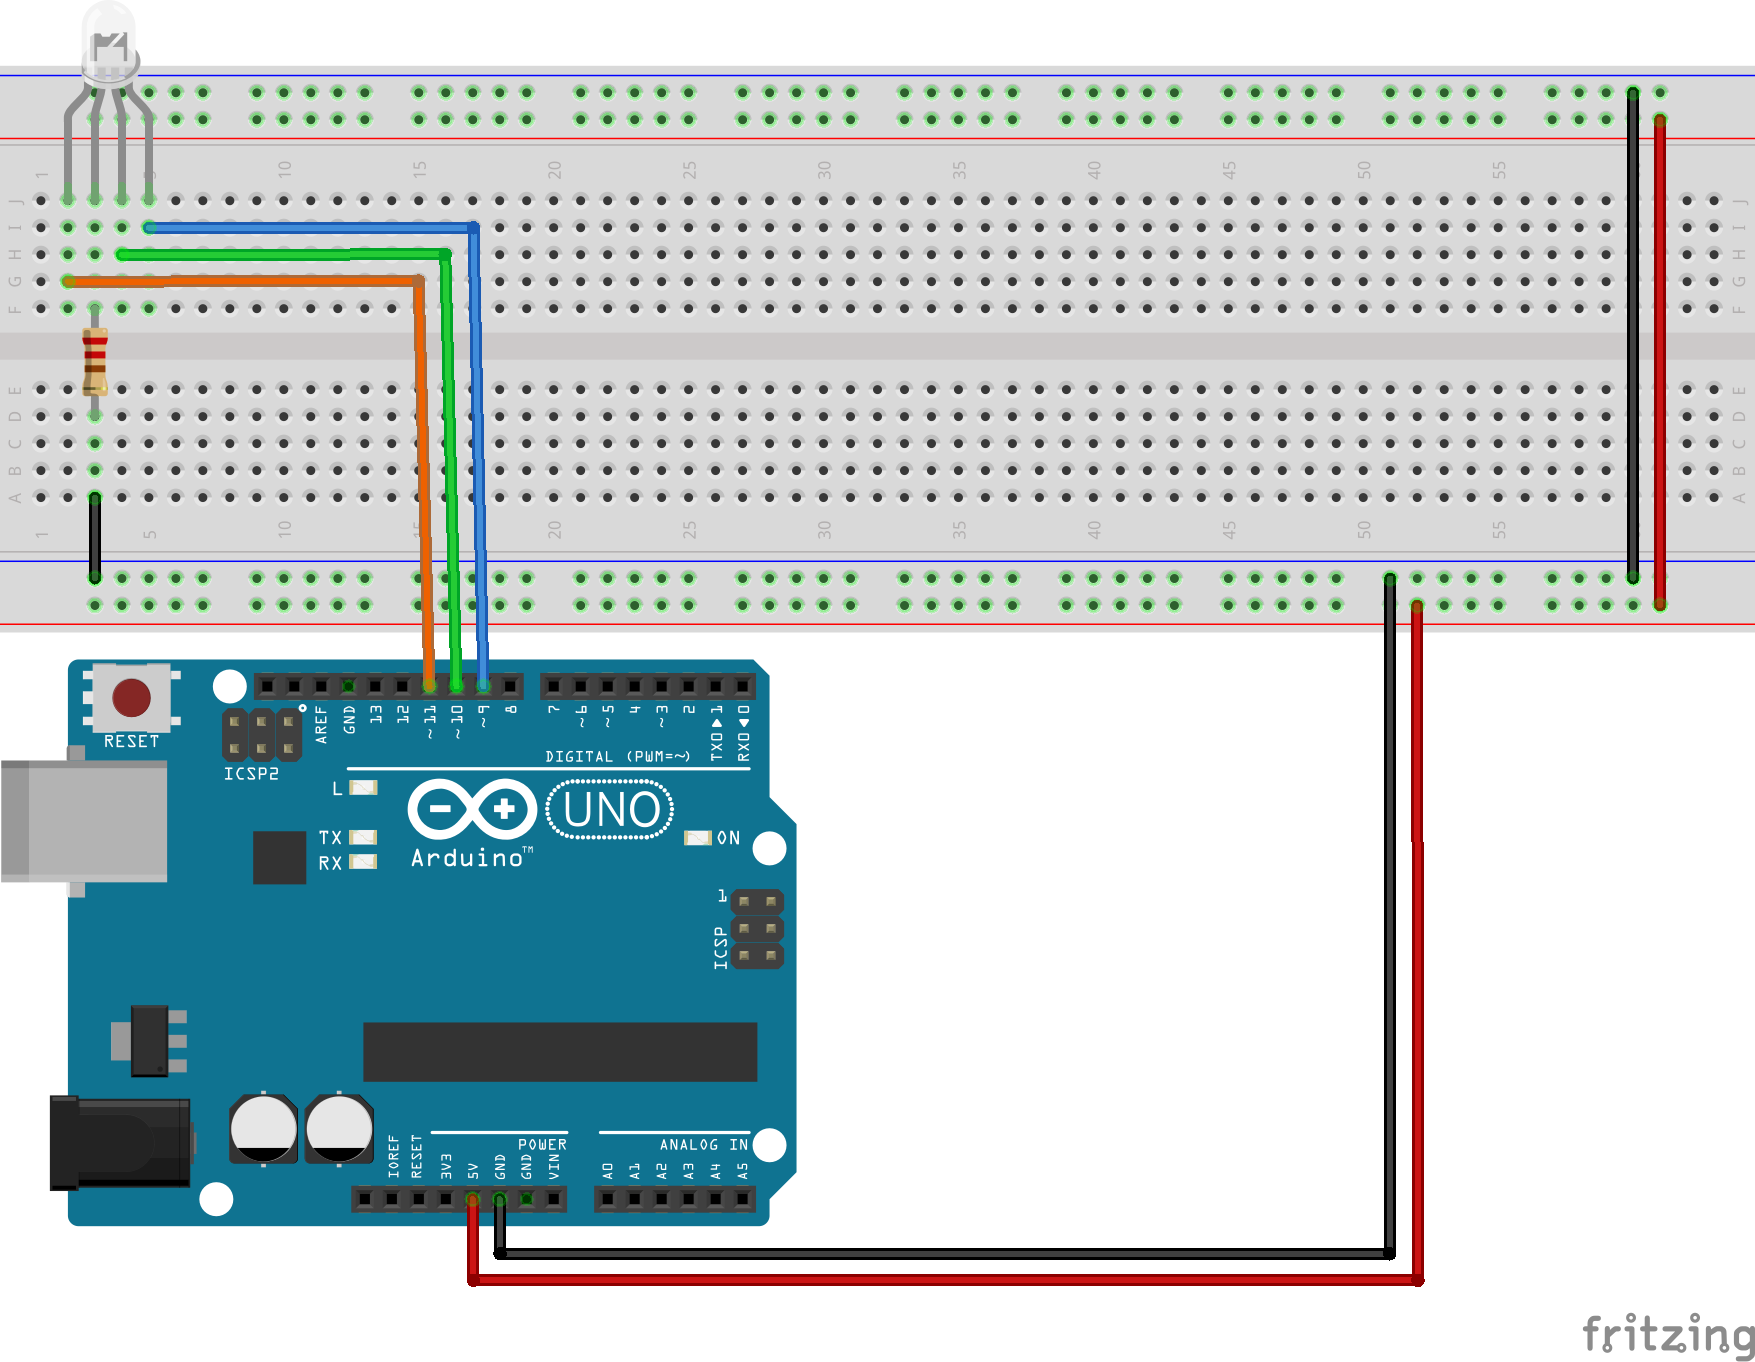
\includegraphics[height=6cm]{img/TP1-2.png}
	\caption{\label{TP1.2}LED RGB}
\end{figure}
%TODO LED RGB

\subsection{Afficheur 7 segments simple}
Dans cette manipulation nous allons connecter un afficheur 7 segments à un notre arduino pour lui faire afficher un compte à rebour allant de 9 à 0. Alternativement nous aurions pu lui faire aire un compte à rebour alant de F (16 en hexadécimal) à 0.
\lstinputlisting[language=C]{Code/TP1/TP1.3/TP1.3.ino}
\begin{figure}[H]
	\centering
	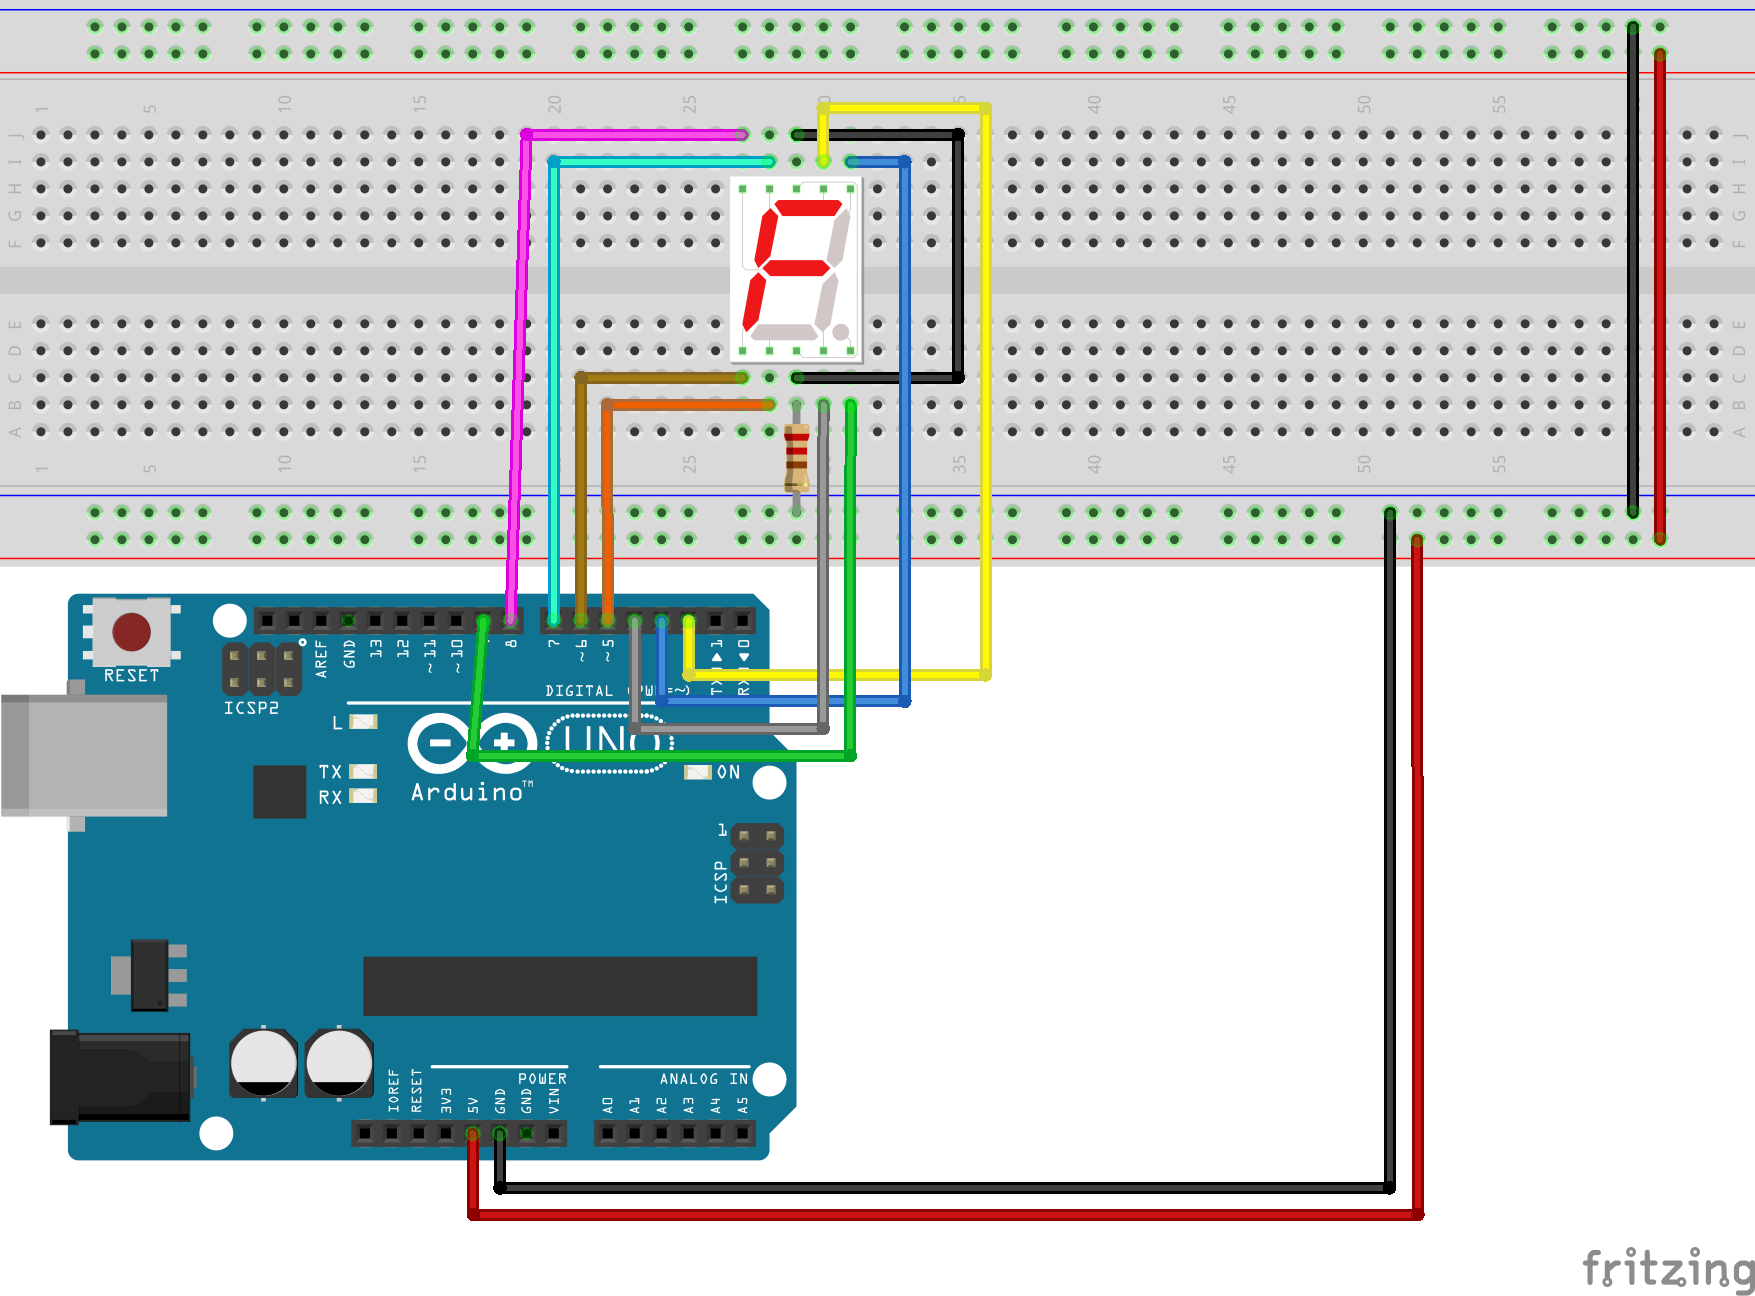
\includegraphics[height=6cm]{img/TP1-3.png}
	\caption{\label{TP1.3}Afficheur 7 segments}
\end{figure}
%TODO 7 Segments

\subsection{Afficheur 7 segments quadruple}
\lstinputlisting[language=C]{Code/TP1/TP1.4/TP1.4.ino}
\begin{figure}[H]
	\centering
	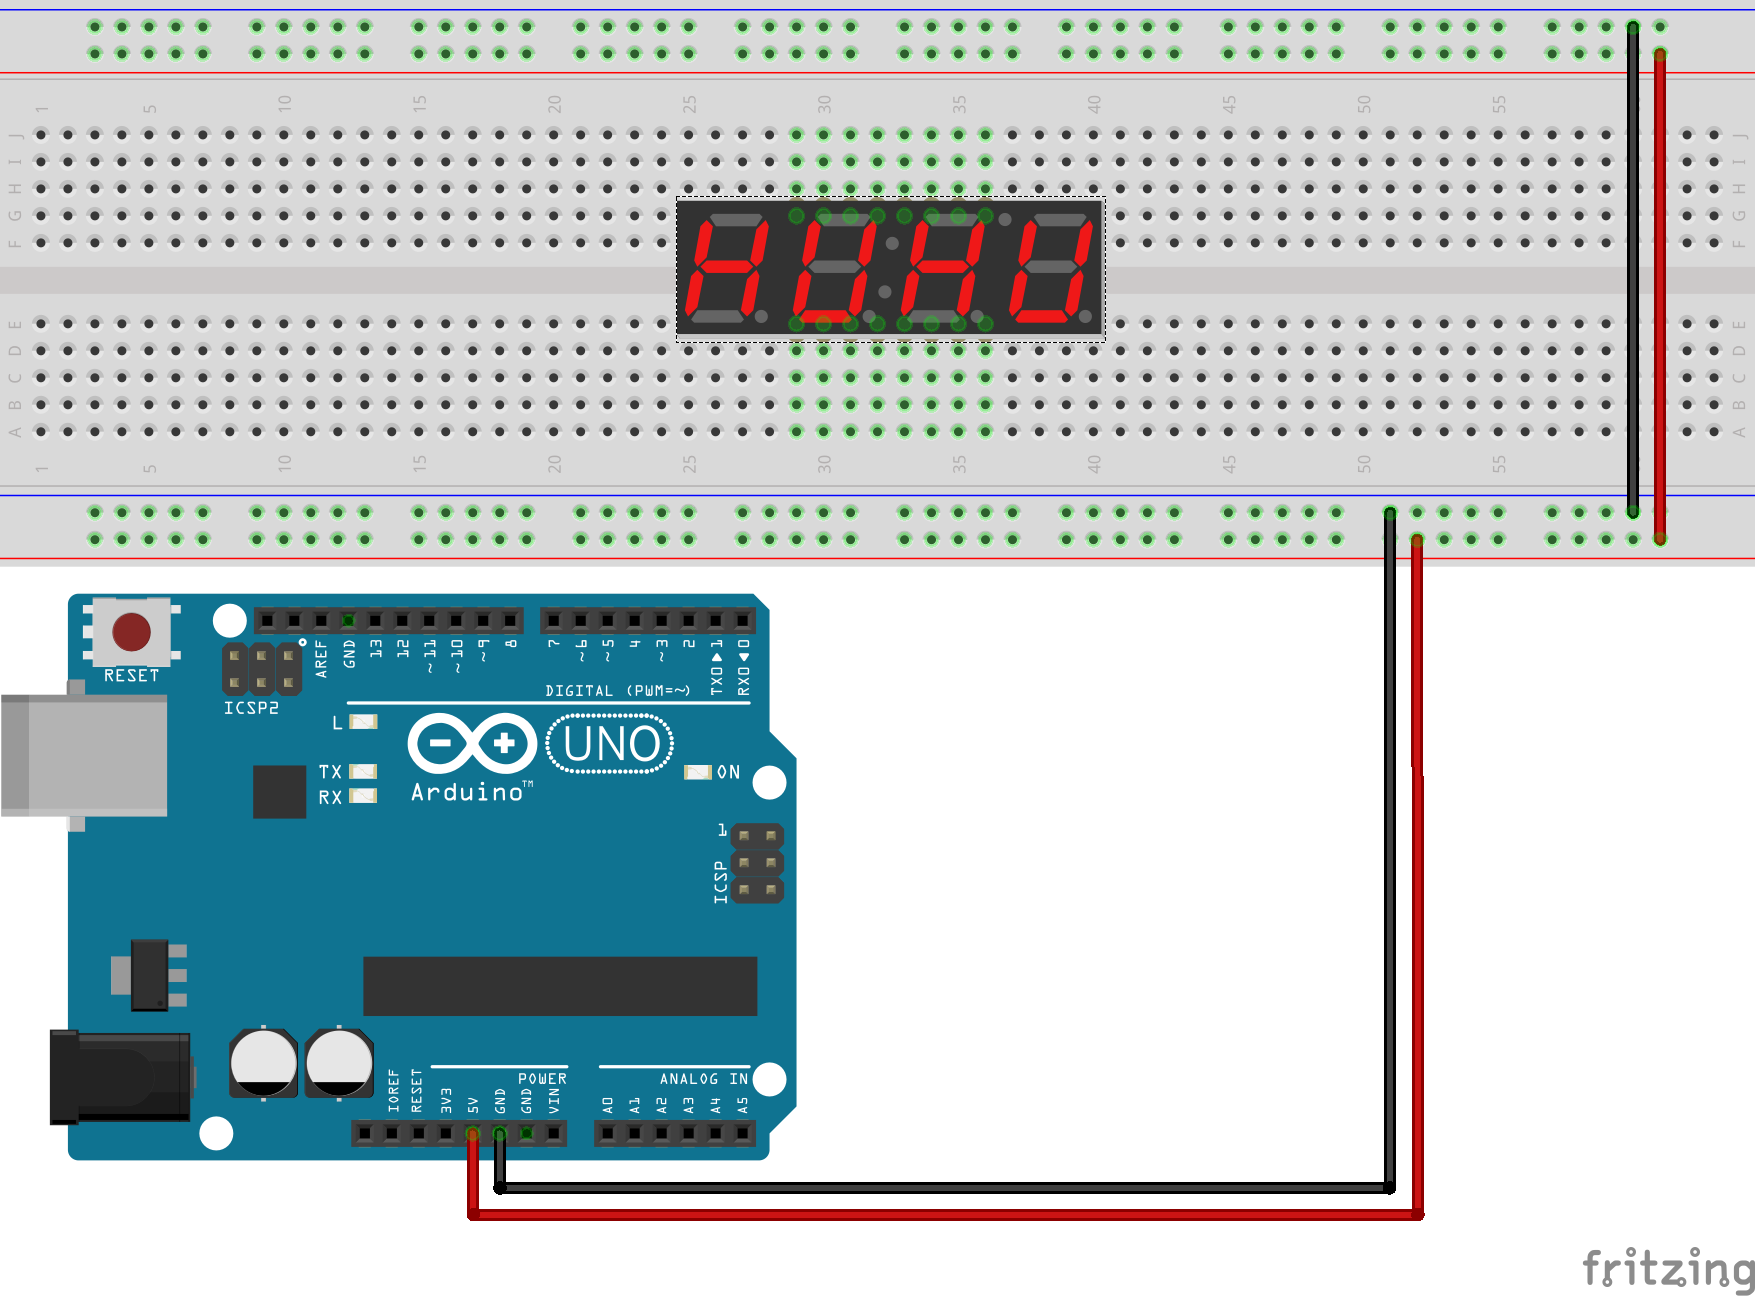
\includegraphics[height=6cm]{img/TP1-4.png}
	\caption{\label{TP1.4}Afficheur 7 segments quadruple}
\end{figure}
%TODO 7 Secgment quadruple

\clearpage
\section{TP2: LCD Time}
\subsection{Objectif}
Dans cette manipulation nous allons apprendre a utiliser un ecran LCD\@. Nous commencerons par decouvrir comment ecrire des phrases simples, puis nous afficherons un texte defillant et enfin nous utiliserons des variables pour afficher l'heure.
\subsection{Matériel}
\begin{itemize}
	\item Un ordinateur
	\item Un arduino Uno R3
	\item Un ecran LCD
	\item Une resistance de 10K$\Omega$
	\item Un potentiometre
\end{itemize}

\subsection{Nom-Prenom}
Le montage est identique pour toutes les manipulations de ce labo. Nous avons utilise la librairie LiquidCrystal, disponnible sur le site officiel d'Arduino. Ici nous allons écrire nos noms sur chacune des lignes de l'écran LCD avec, à gauche, le numéro de notre groupe. Nous utilsons la librairie LiquidCrystal qui nous permet de facilement afficher du texte sur notre écran LCD\@.
\lstinputlisting[language=C]{Code/TP2/TP2.1/TP2.1.ino}
\begin{figure}[H]
	\centering
	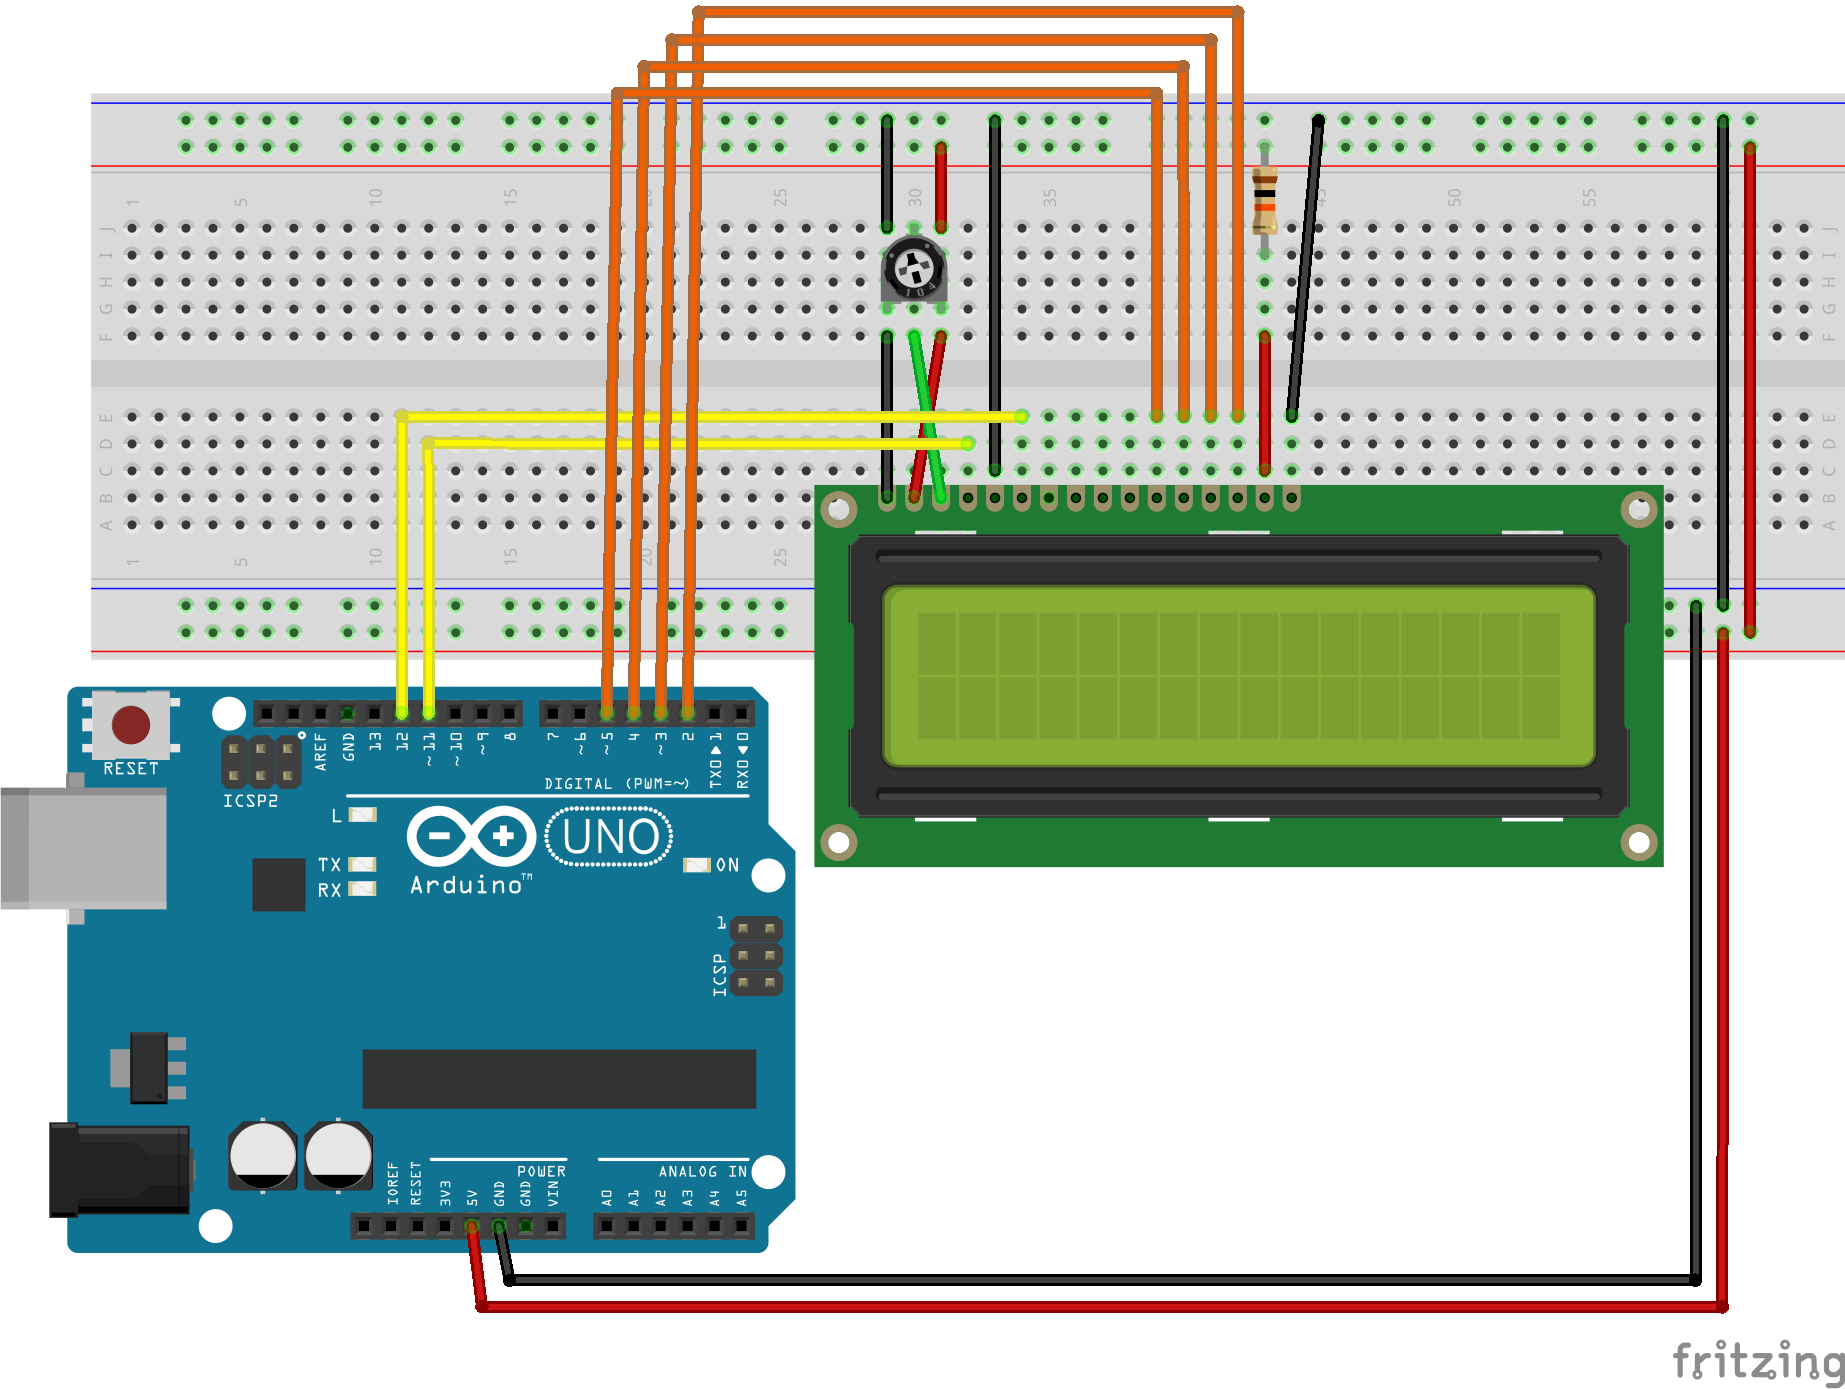
\includegraphics[height=6cm]{img/TP2-1.png}
	\caption{\label{TP2.1}Nom-Prenom}
\end{figure}
%TODO Ecran LCD

\subsection{Texte deroulant}
Dans cette manipulation nous allons afficher un texte déroulant vers la gauche.
\lstinputlisting[language=C]{Code/TP2/TP2.2/TP2.2.ino}

\subsection{Horloge}
Dans cette manipulation nous allons afficher une horloge au milieu de la deuxième ligne de l'écran. Une fois téléversé, l'Arduino commencera a afficher l'heure à 22h59m50 car il n'est pas possible d'afficher l'heure réelle sans utiliser des boutons pour régler l'heure ou un module \textit{Real Time Clock}.
\lstinputlisting[language=C]{Code/TP2/TP2.3/TP2.3.ino}

\subsection{Decompte}
De la même façon que nous avons affiché l'heure nous affichons ici un décompte qui part de 9999 jusu'à 0.
\lstinputlisting[language=C]{Code/TP2/TP2.4/TP2.4.ino}

\clearpage
\section{TP3: Push Push}
\subsection{Objectif}
Dans cette manipulation nous allons voir comment faire intéragir des modules d'entrées avec des modules de sortie pour par exemple, allumer une LED par appuis sur un bouton, afficher le une valeur correspondant à un bouton sur un matrice ou encore faire intéragie une matrice de led avec un joystick.
\
subsection{Matériel}a
\begin{itemize}
	\item Un ordinateur
	\item Un arduino Uno R3
	\item Un boutton poussoir
	\item Des resistance de 10K$\Omega$
	\item Une led
	\item Une matrice de boutons
	\item Un afficheur LCD
	\item Un Joystick
	\item Une matrice de LED
\end{itemize}


\subsection{LED et boutton}

\lstinputlisting[language=C]{Code/TP3/TP3.1/TP3.1.ino}
\begin{figure}[H]
	\centering
	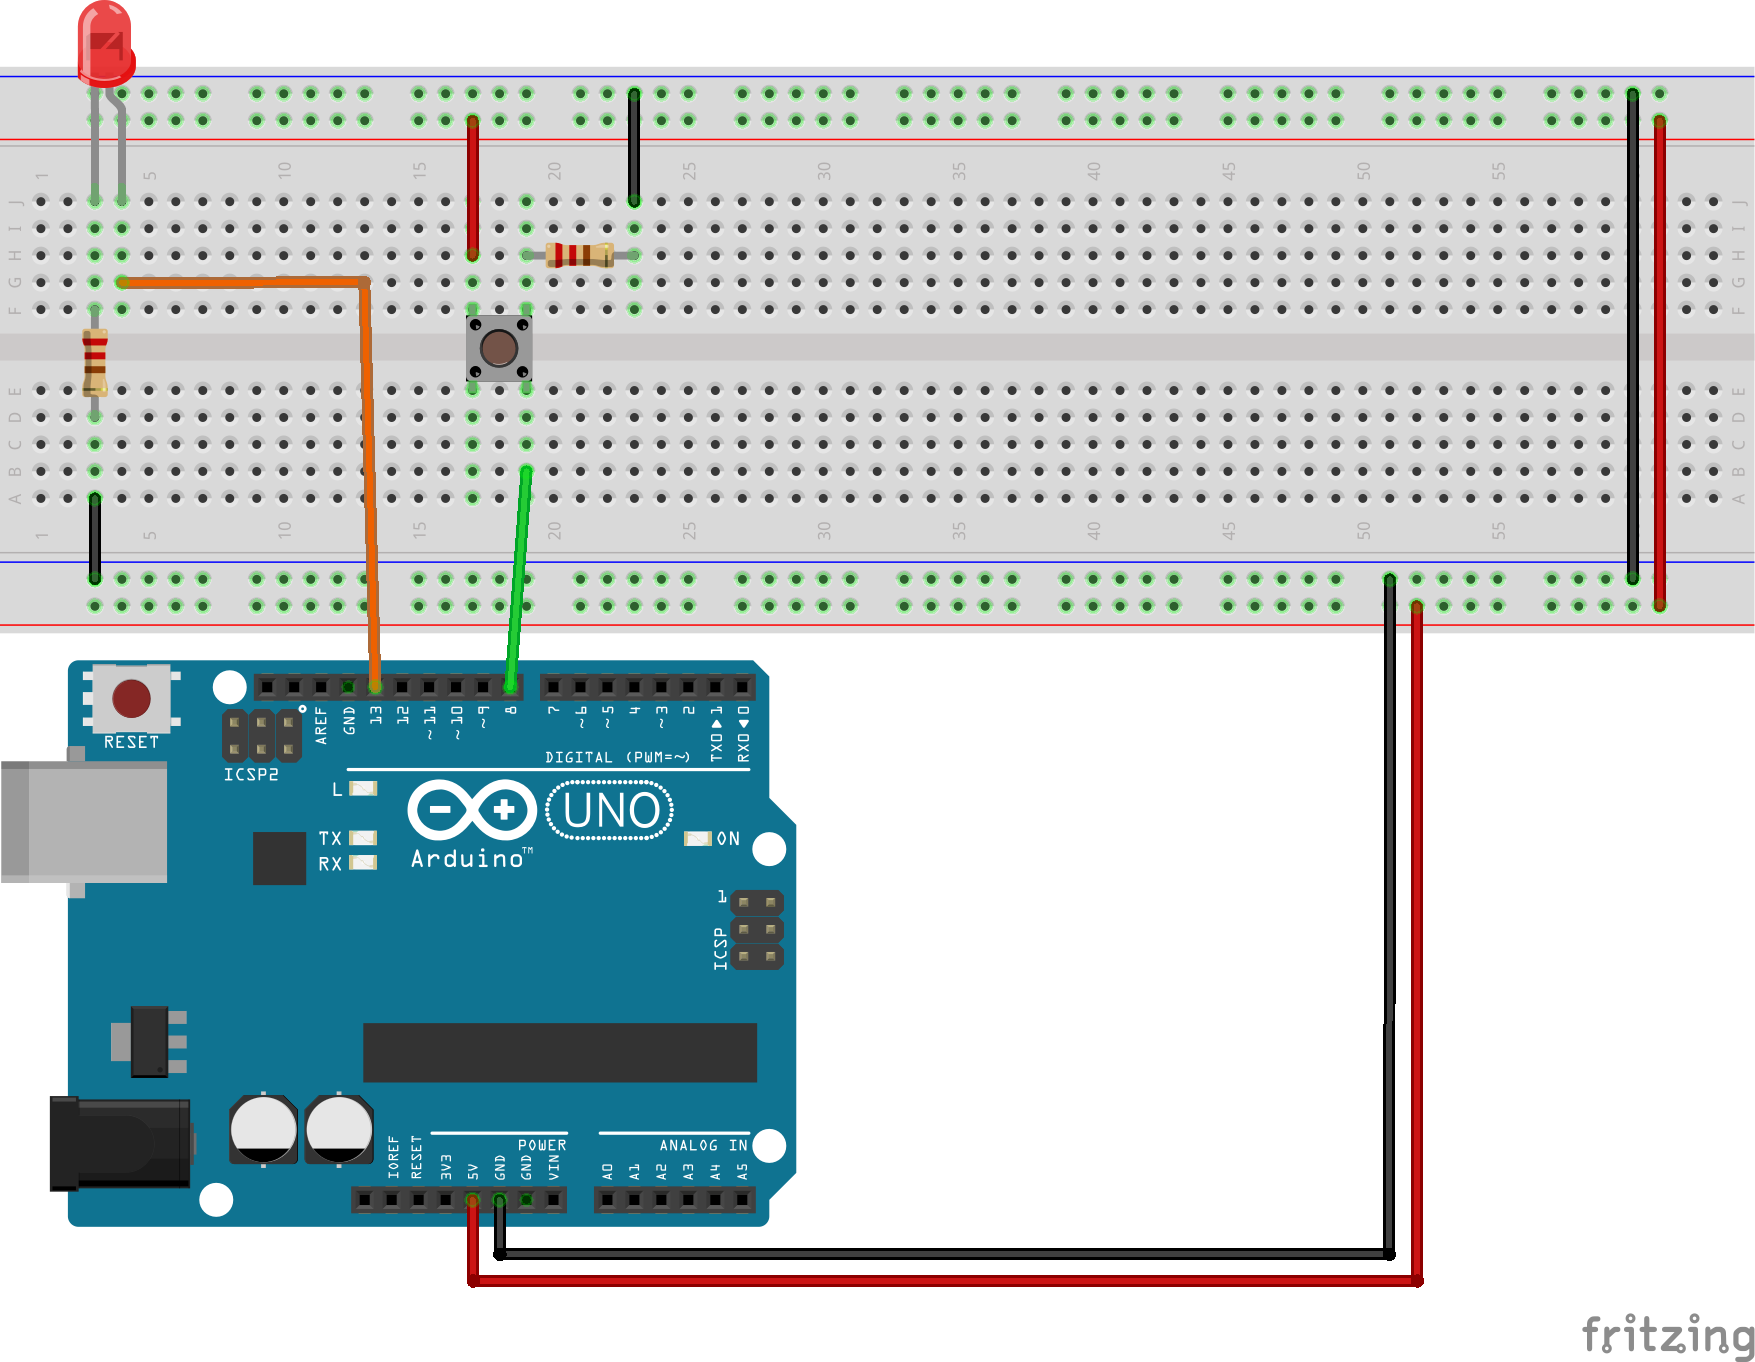
\includegraphics[height=6cm]{img/TP3-1.png}
	\caption{\label{TP3.1}LED et boutton}
\end{figure}
%TODO Button

\subsection{Debounce}

\lstinputlisting[language=C]{Code/TP3/TP3.2/TP3.2.ino}
\begin{figure}[H]
	\centering
	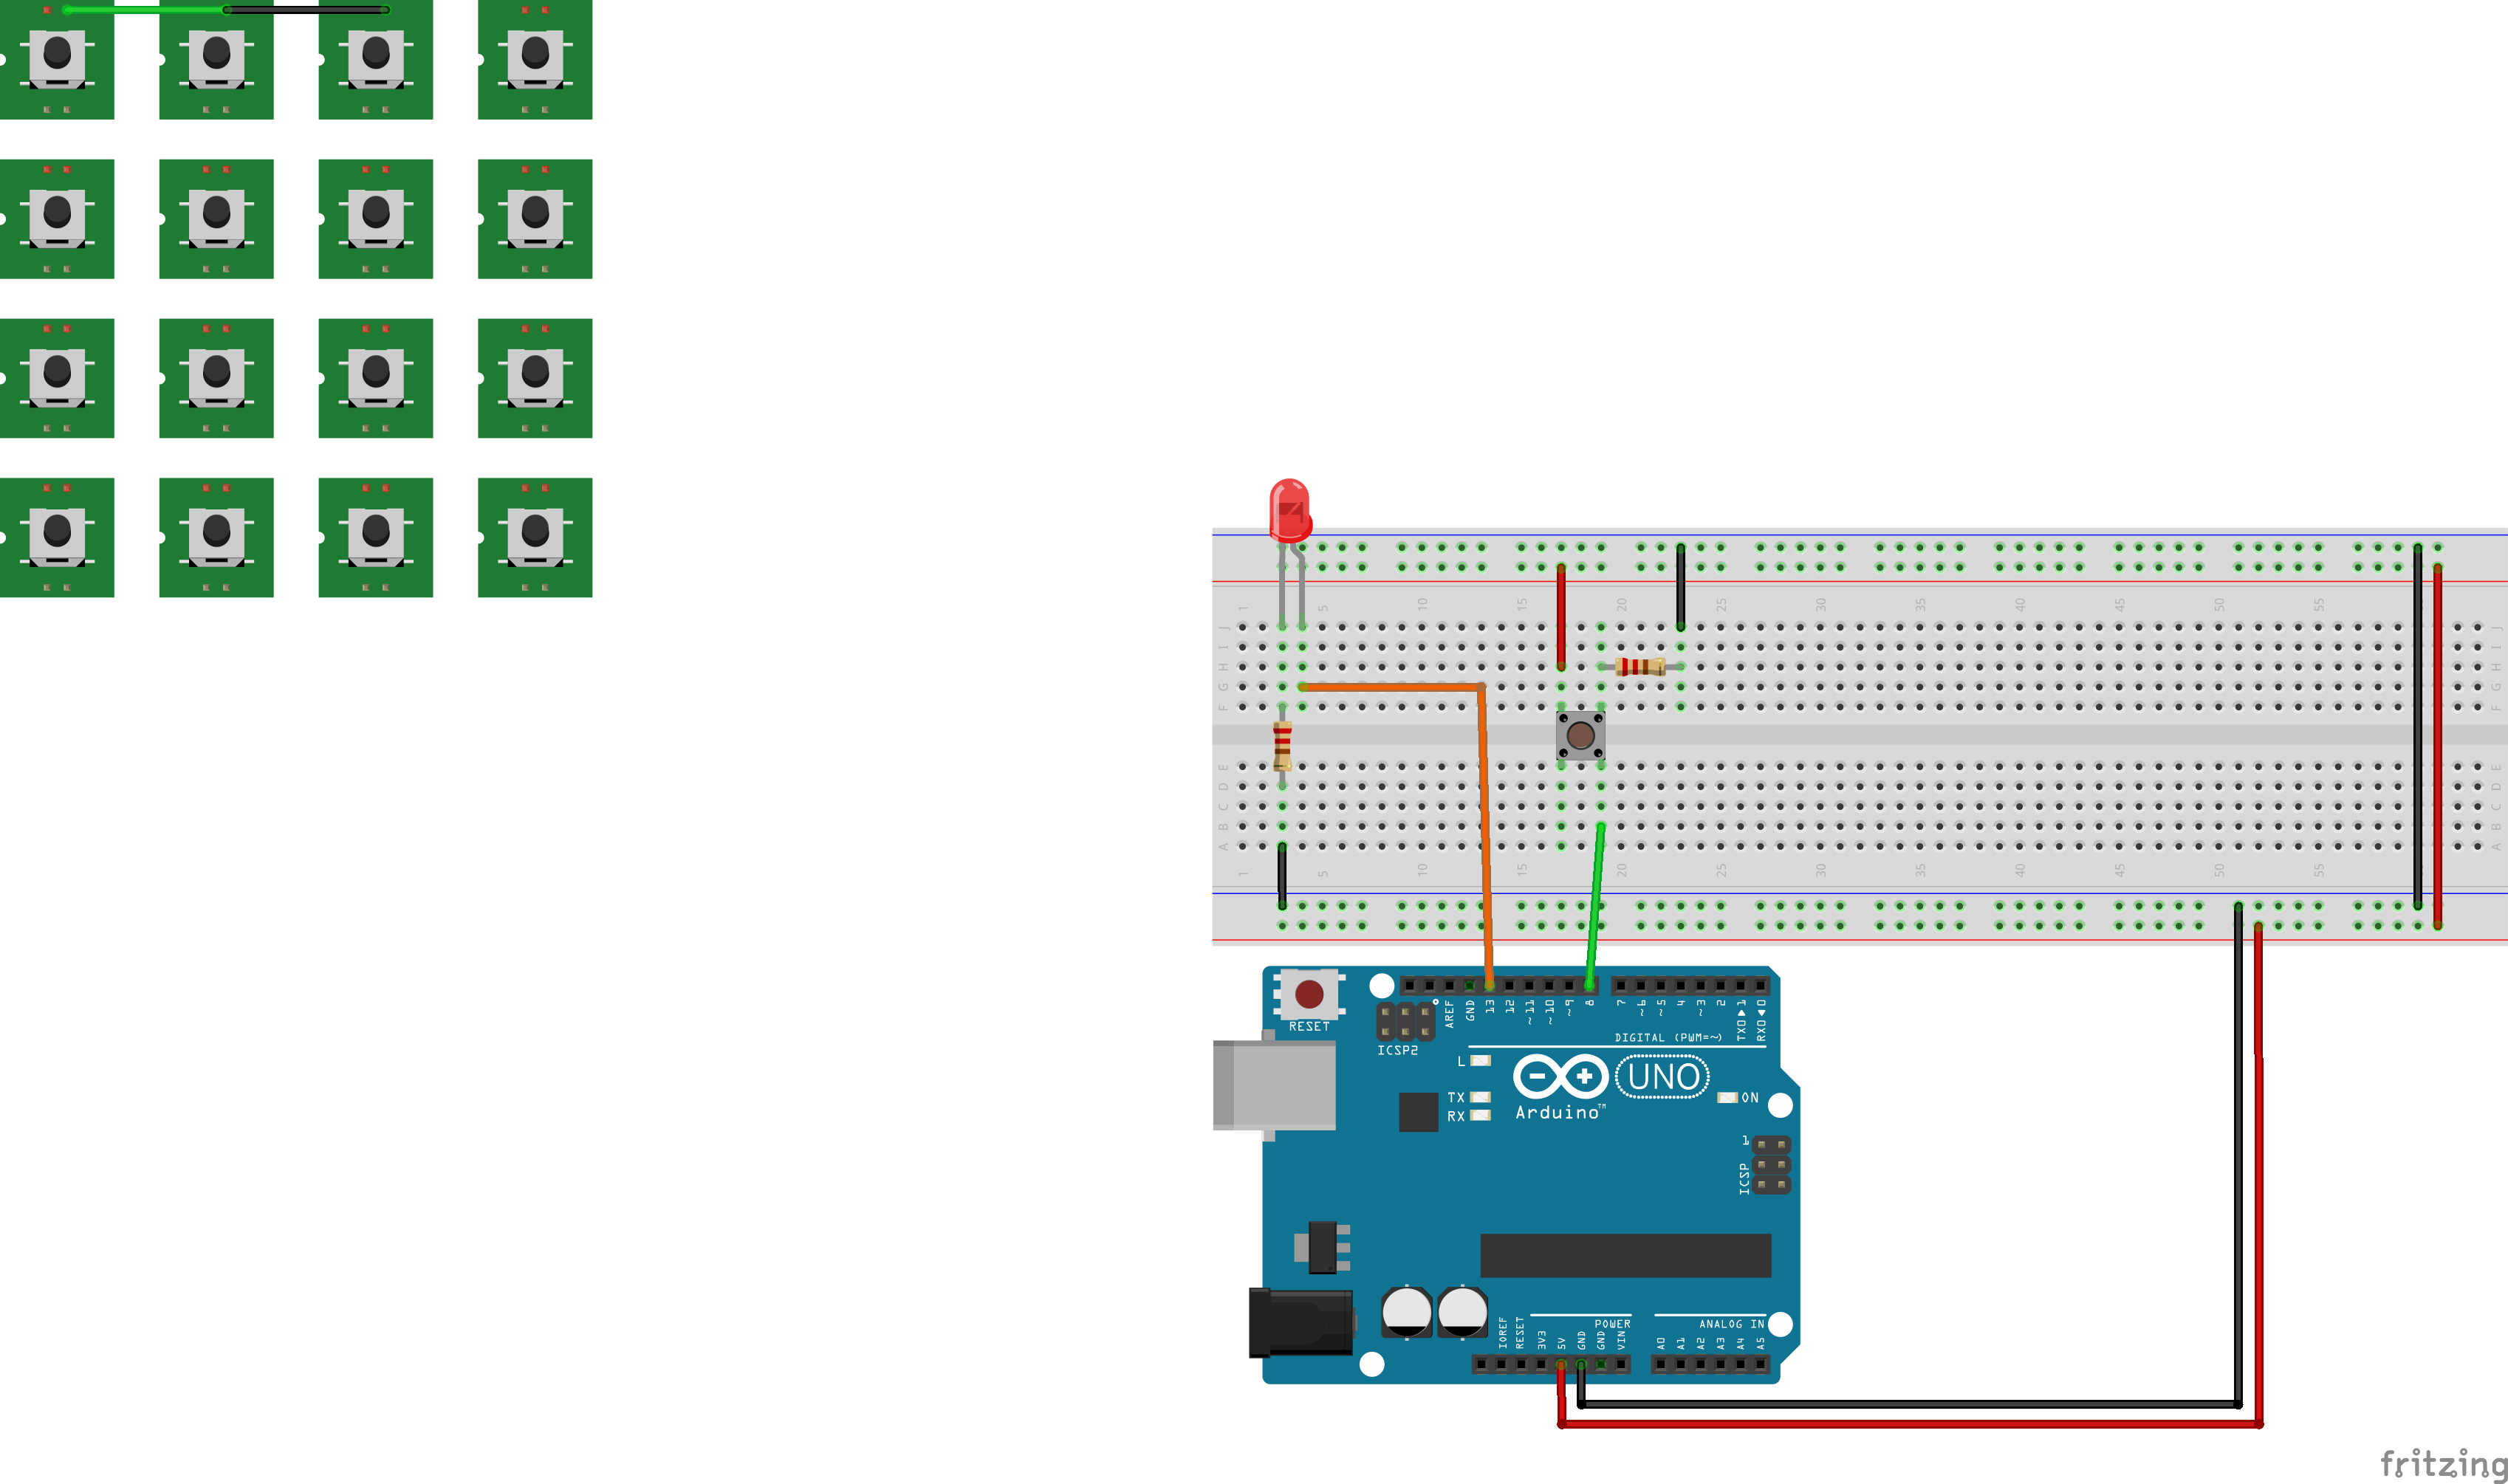
\includegraphics[height=6cm]{img/TP3-2.png}
	\caption{\label{TP3.2}Debounce}
\end{figure}
\subsection{Matrice de bouttons}

\lstinputlisting[language=C]{Code/TP3/TP3.3/TP3.3.ino}
\begin{figure}[H]
	\centering
	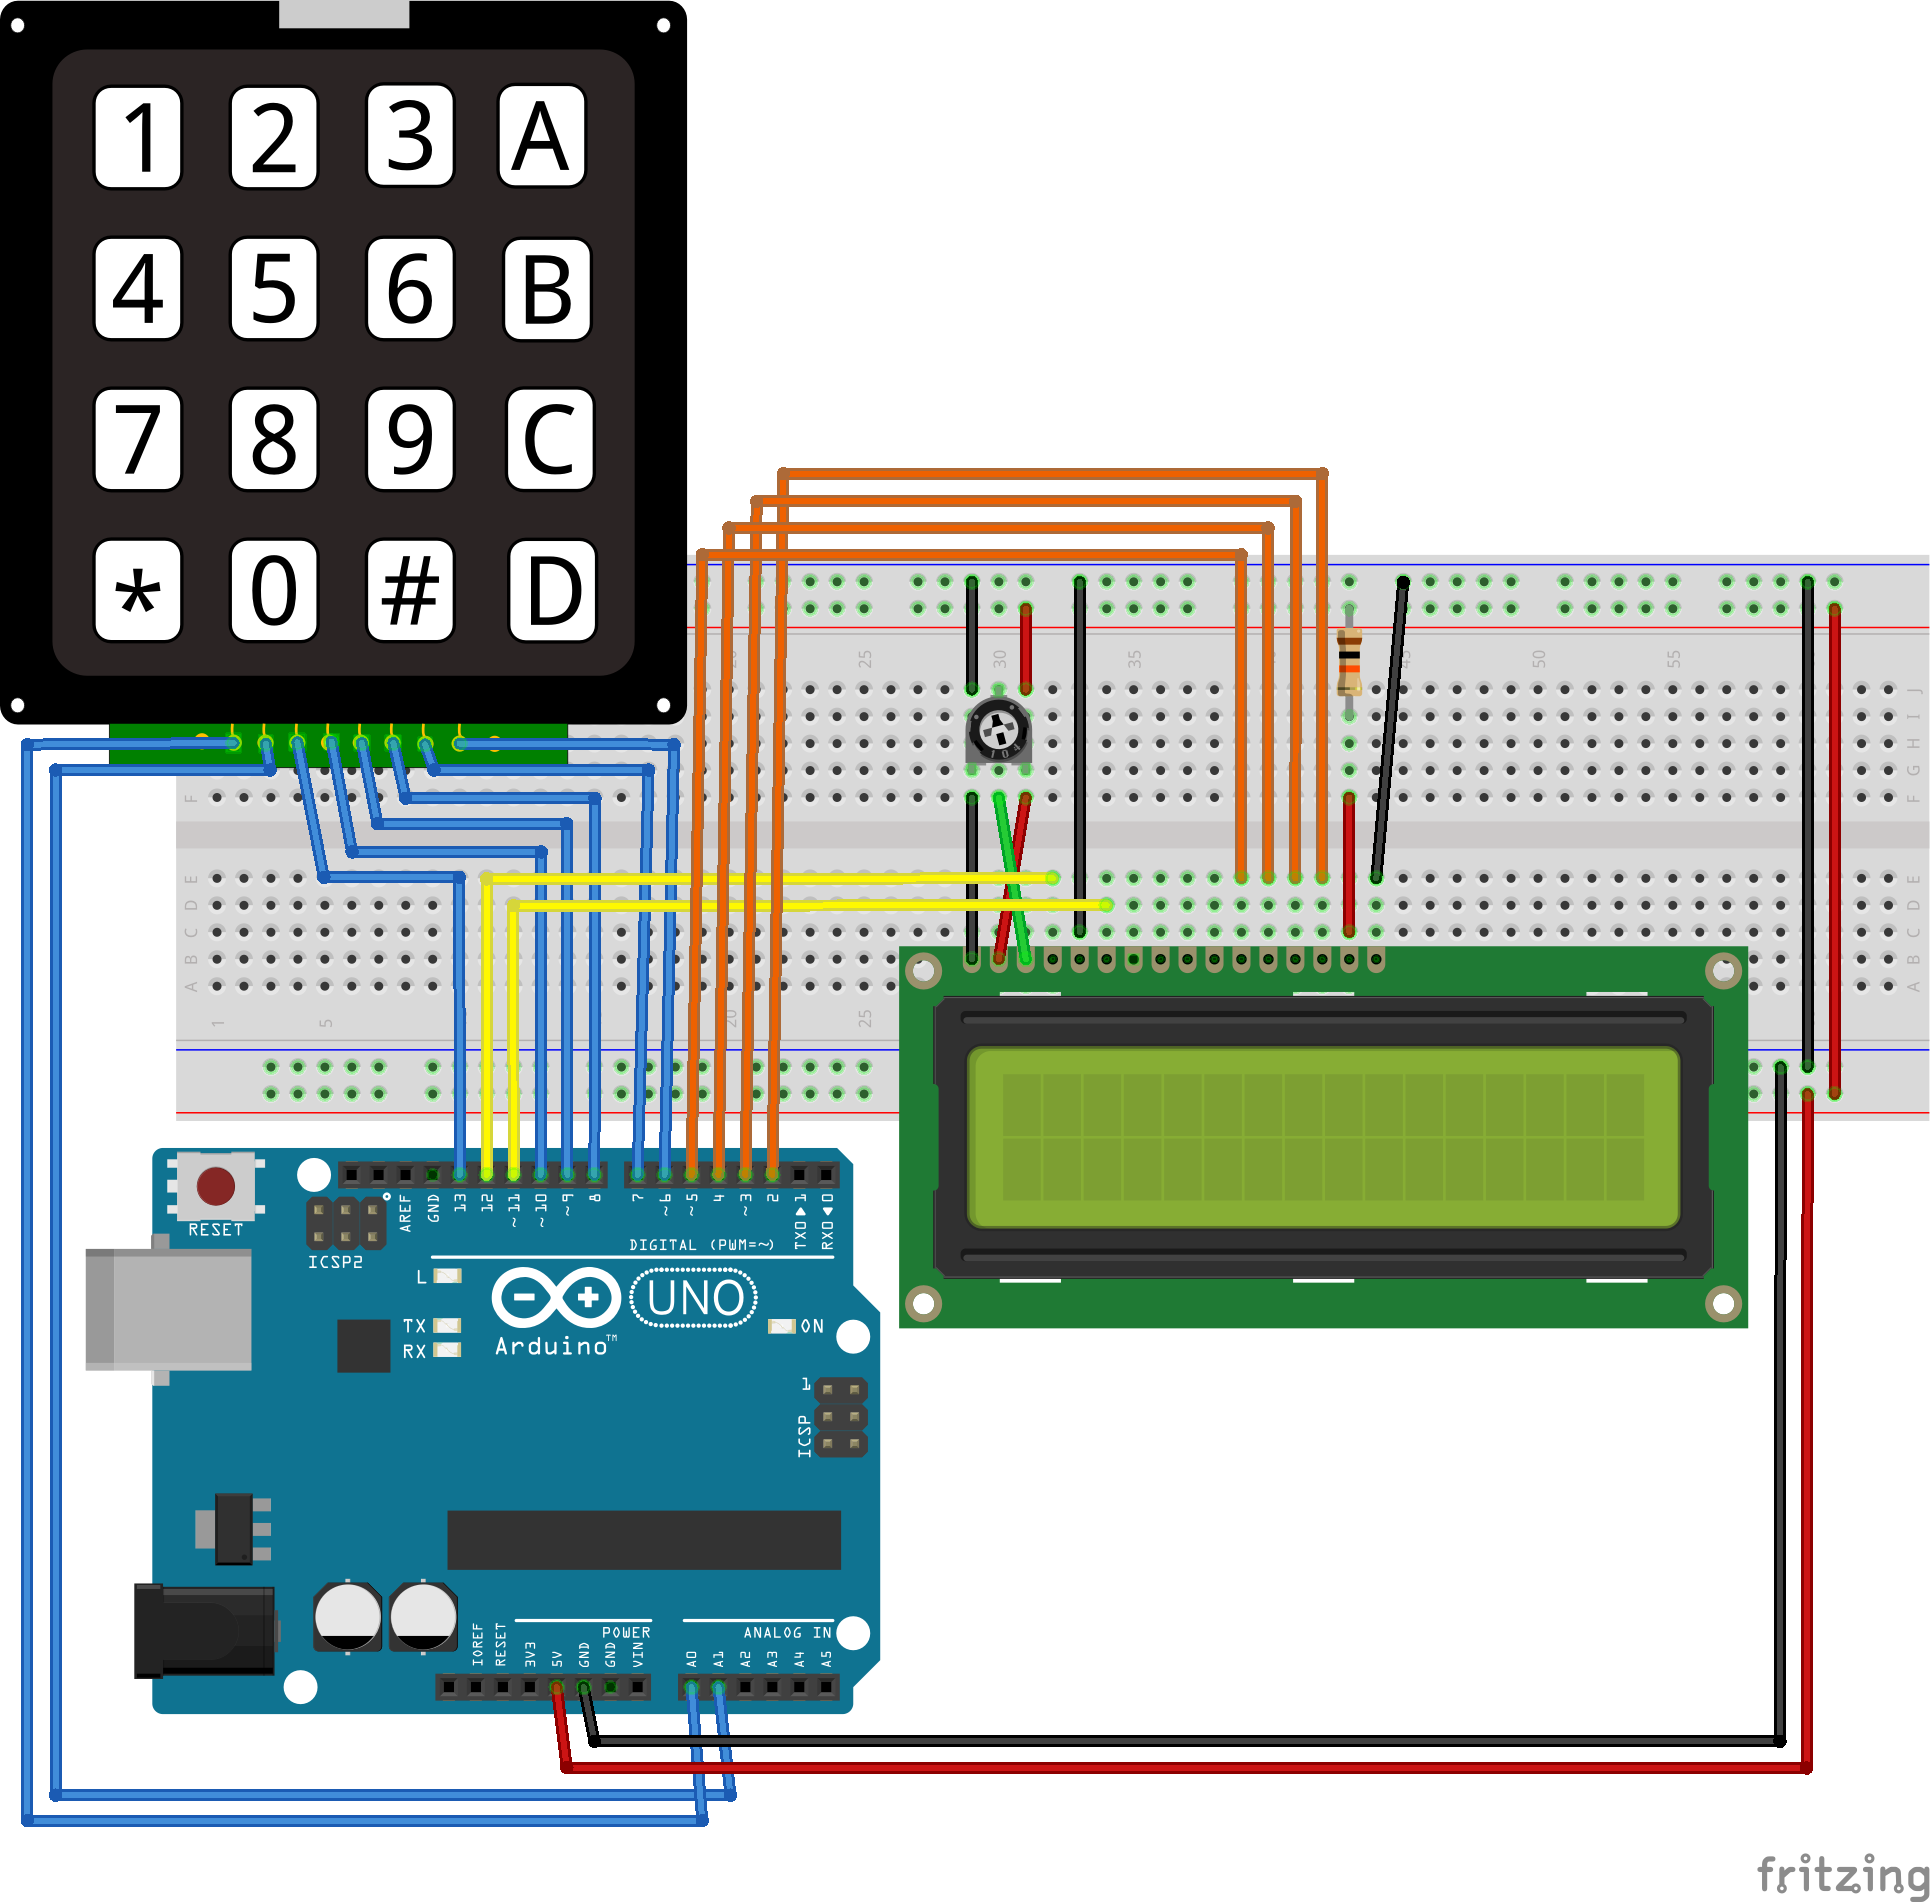
\includegraphics[height=6cm]{img/TP3-3.png}
	\caption{\label{TP3.3}Matrice de bouttons}
\end{figure}

% \subsection{Joystick et matrice de LED}

% \lstinputlisting[language=C]{Code/TP3/TP3.4/TP3.4.ino}
% \begin{figure}[H]
% 	\centering
% 	\includegraphics[height=6cm]{img/TP3-4.png}
% 	\caption{\label{TP3.4}Joystick et matrice de LED}
% \end{figure}
%%TODO Matrice button

\clearpage
\section{TP4: IR}
\subsection{Objectif}
Dans cette manipulation nous allons voir comment utiliser une télécommande infra rouge et un récepteur infra rouge pour controller des modules à une distance pouvant aller jusqu'a 10 metres. Nous allons donc controller une LED, la couleur d'une LED RGB ainsi qu'un moteur.
\subsection{Matériel}
\begin{itemize}
	\item Un ordinateur
	\item Un arduino Uno R3
	\item Un récepteur IR
	\item Des resistance de 10K$\Omega$
	\item Une led
	\item Une LED RGB
	\item Un Un moteur avec controlleur
\end{itemize}

\subsection{Controle d'une LED à distance}

\lstinputlisting[language=C]{Code/TP4/TP4.1/TP4.1.ino}
\begin{figure}[H]
	\centering
	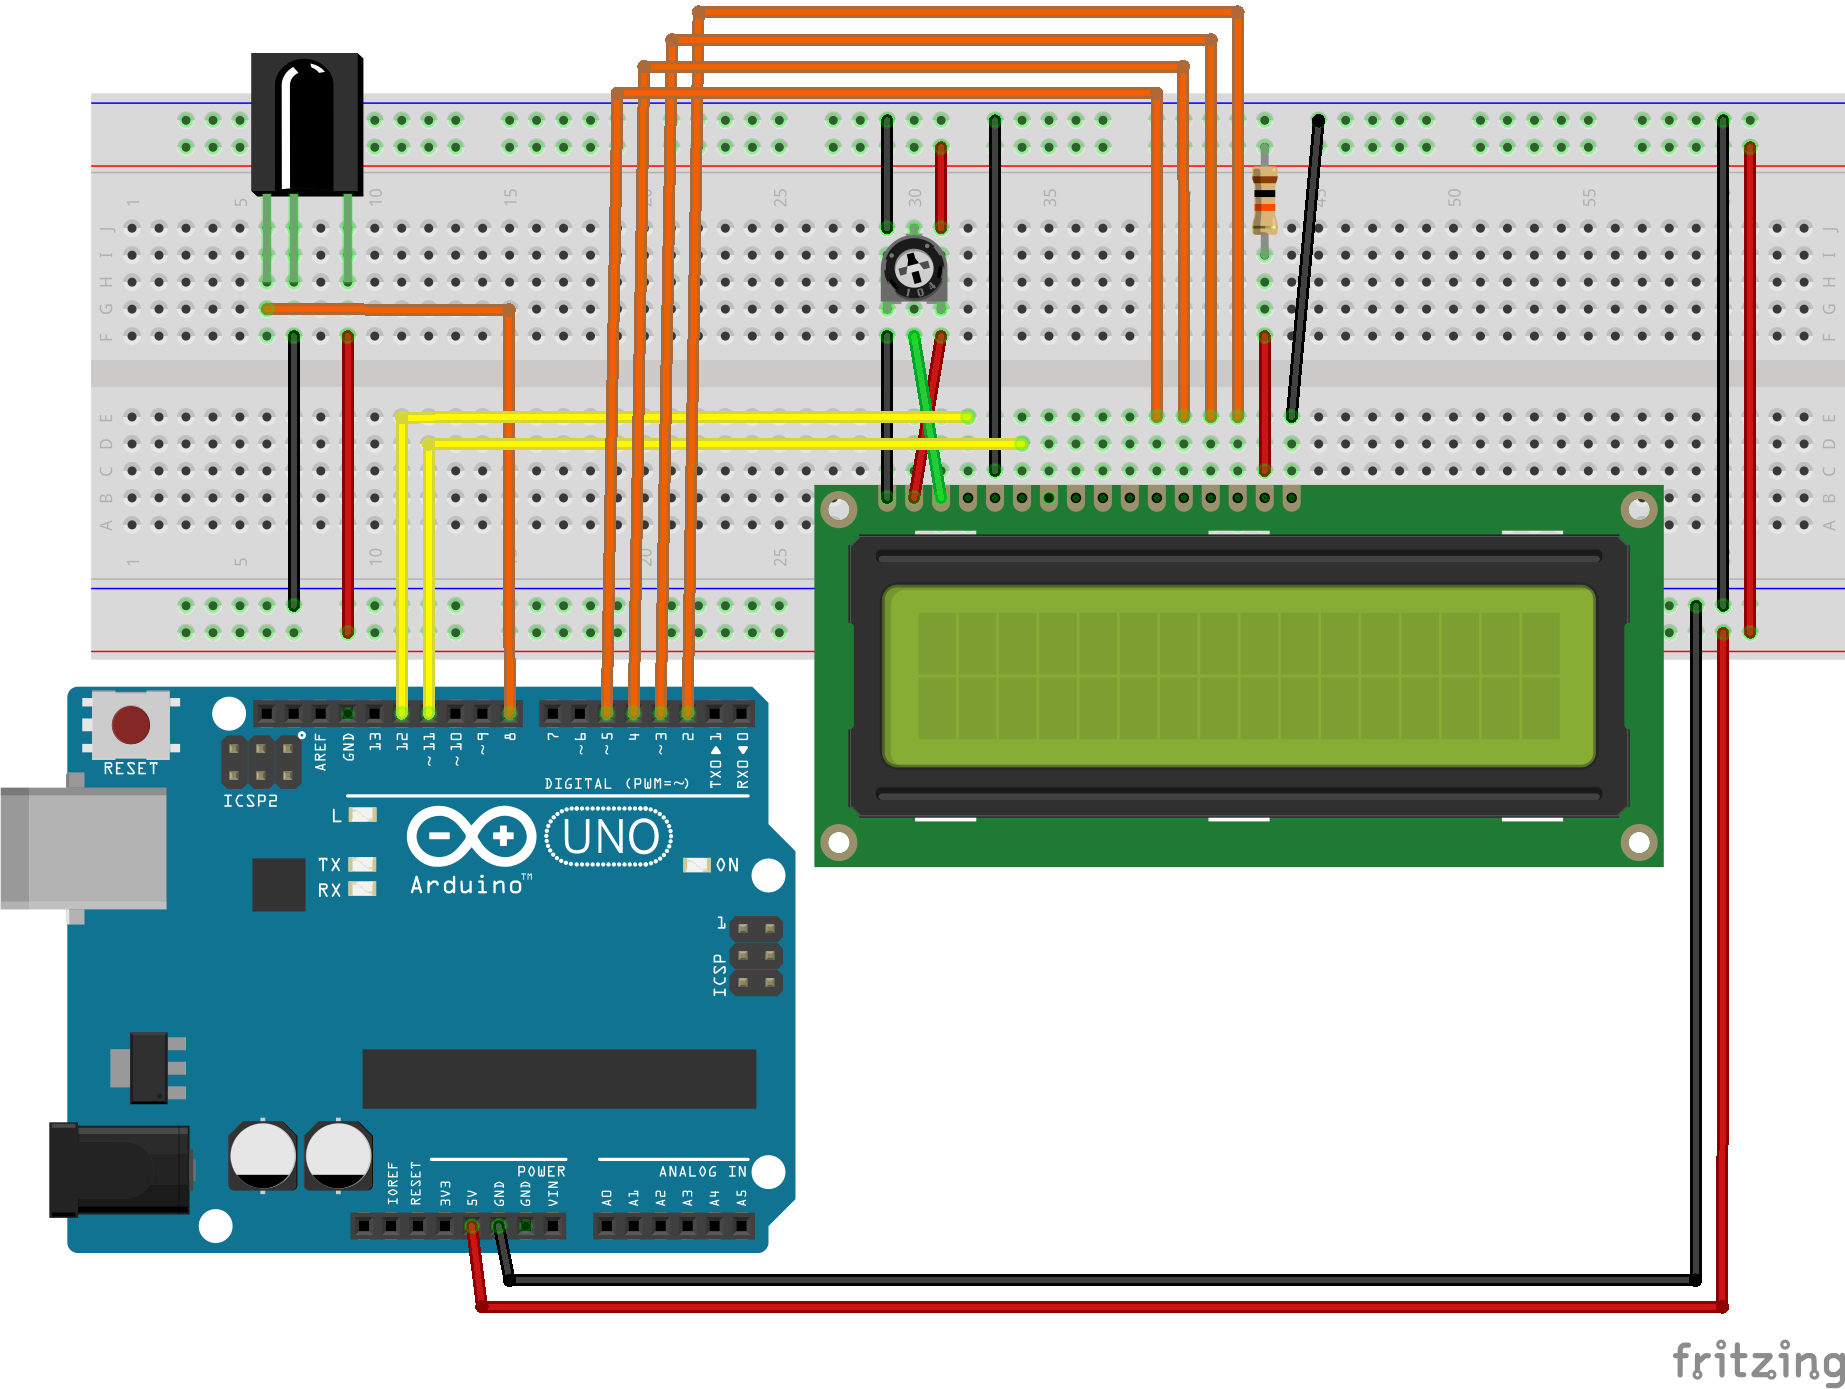
\includegraphics[height=6cm]{img/TP4-1.png}
	\caption{\label{TP4.1}Controle d'une LED}
\end{figure}


\subsection{Controle de la couleur d'une LED RGB à distance}

\lstinputlisting[language=C]{Code/TP4/TP4.2/TP4.2.ino}
\begin{figure}[H]
	\centering
	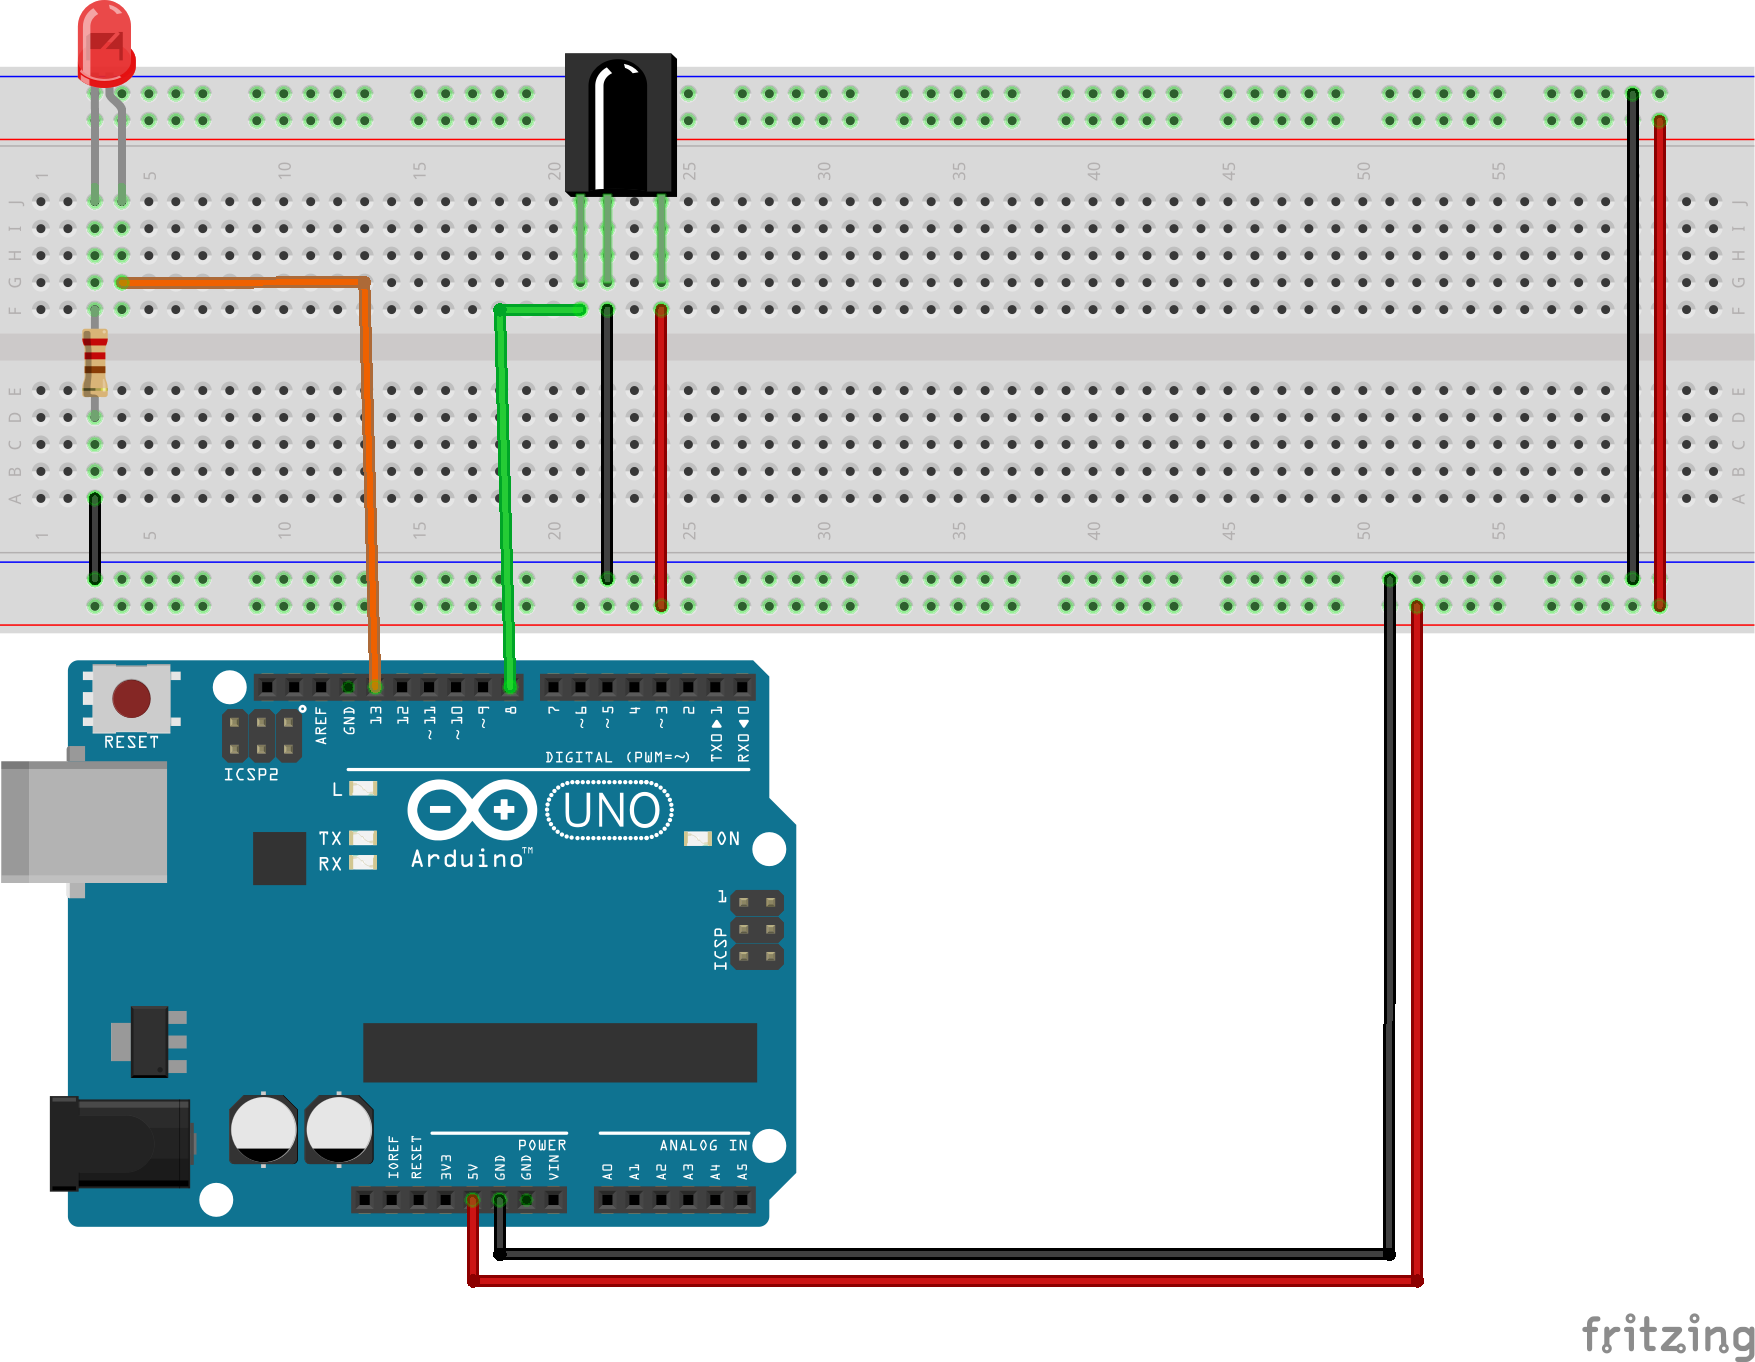
\includegraphics[height=6cm]{img/TP4-2.png}
	\caption{\label{TP4.2}Controle d'une LED RGB à distance}
\end{figure}

\subsection{Controle d'un moteur à distance}

\lstinputlisting[language=C]{Code/TP4/TP4.3/TP4.3.ino}
\begin{figure}[H]
	\centering
	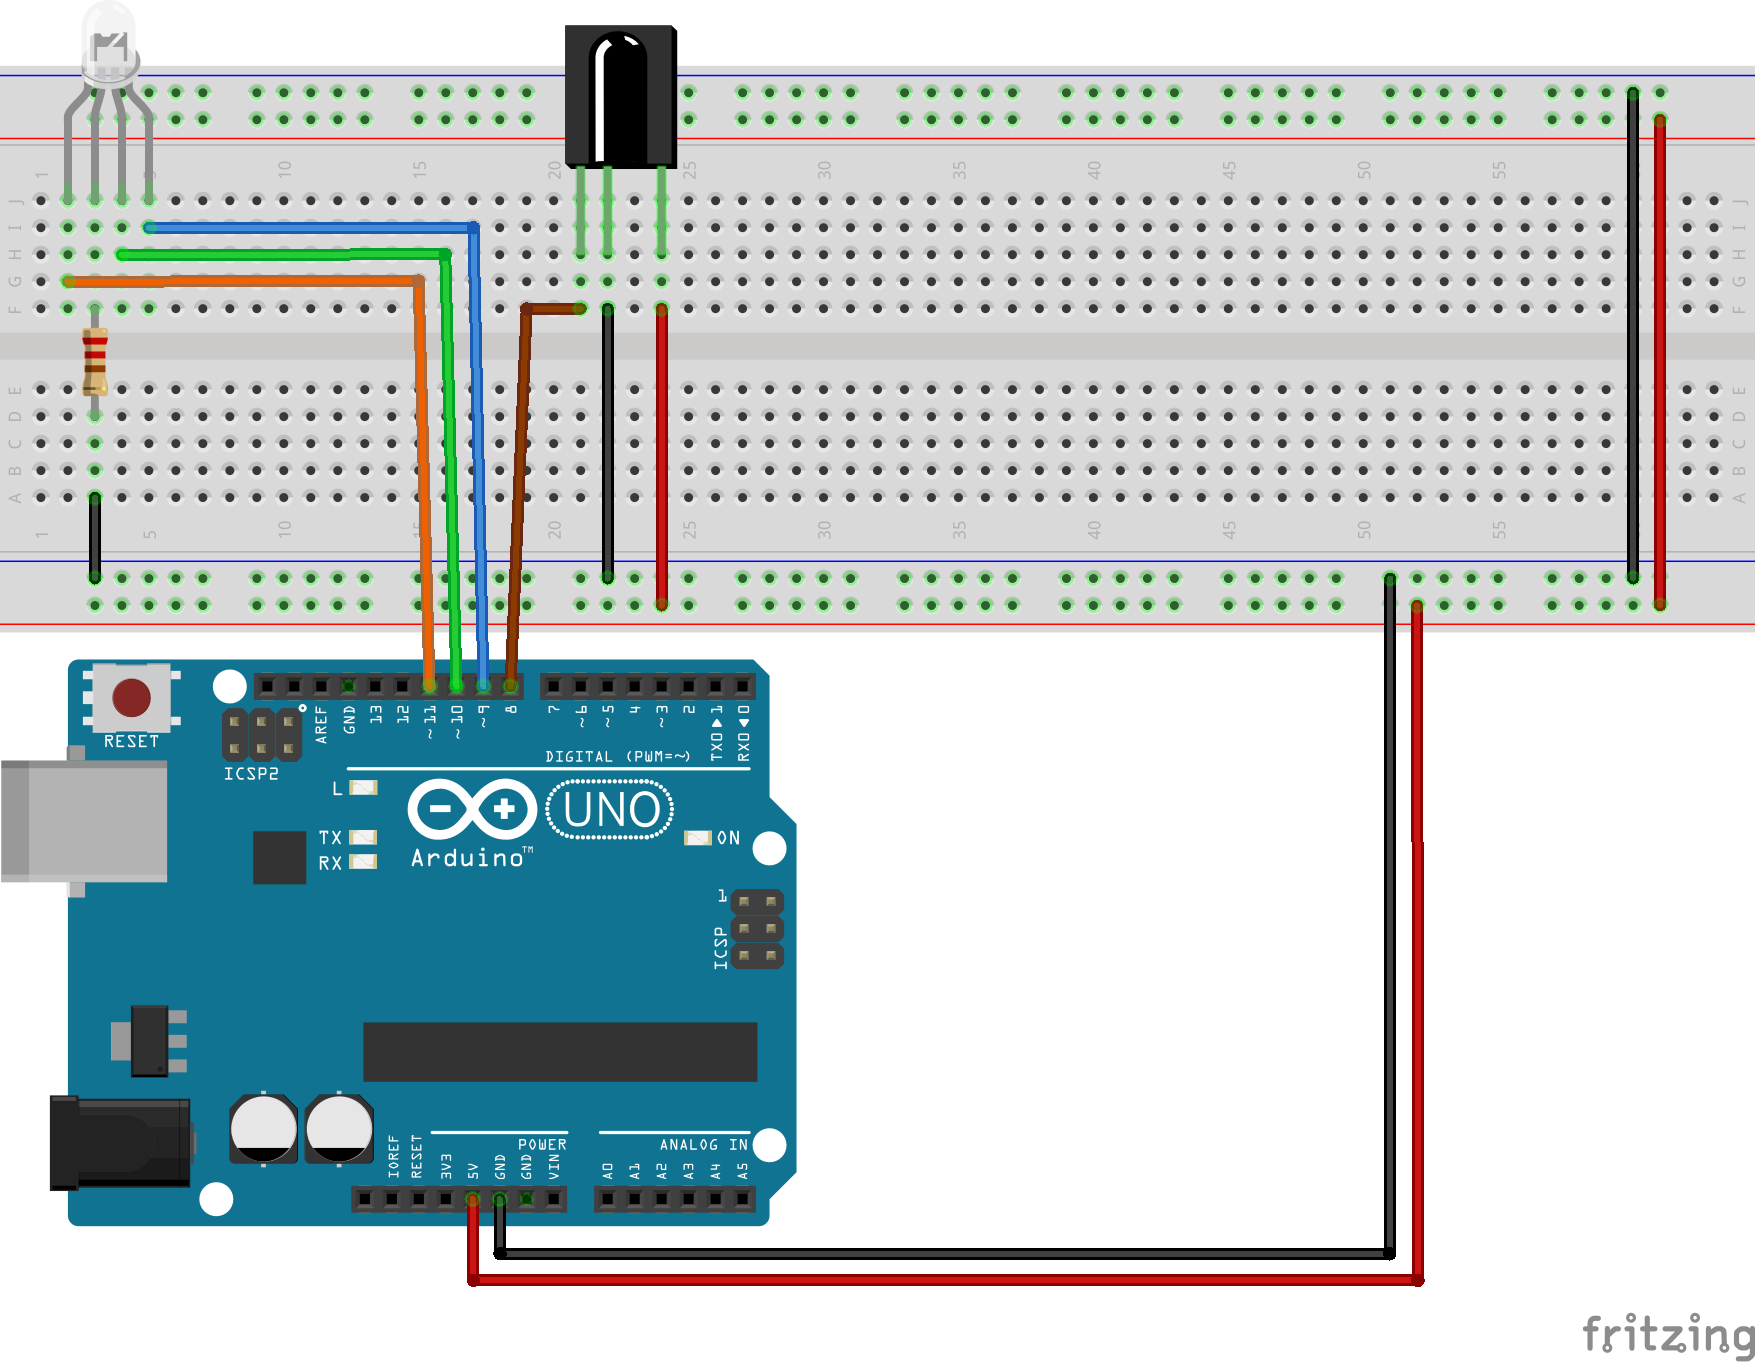
\includegraphics[height=6cm]{img/TP4-3.png}
	\caption{\label{TP4.3}Controle d'un moteur à distance}
\end{figure}

% \subsection{Joystick et matrice de LED}

% \lstinputlisting[language=C]{Code/TP3/TP3.4/TP3.4.ino}
% \begin{figure}[H]
% 	\centering
% 	\includegraphics[height=6cm]{img/TP3-4.png}
% 	\caption{\label{TP3.4}Joystick et matrice de LED}
% \end{figure}

\clearpage
\section{TP5: Motors}
\subsection{Objectif}
Dans cette manipulation nous allons voir comment faire intéragir des modules d'entrées avec des modules de sortie pour par exemple, allumer une LED par appuis sur un bouton, afficher le une valeur correspondant à un bouton sur un matrice ou encore faire intéragie une matrice de led avec un joystick.
\subsection{Matériel}a
\begin{itemize}
	\item Un ordinateur
	\item Un arduino Uno R3
	\item Un boutton poussoir
	\item Des resistance de 10K$\Omega$
	\item Une led
	\item Une matrice de boutons
	\item Un afficheur LCD
	\item Un Joystick
	\item Une matrice de LED
\end{itemize}

\subsection{LED et boutton}

\lstinputlisting[language=C]{Code/TP3/TP3.1/TP3.1.ino}
\begin{figure}[H]
	\centering
	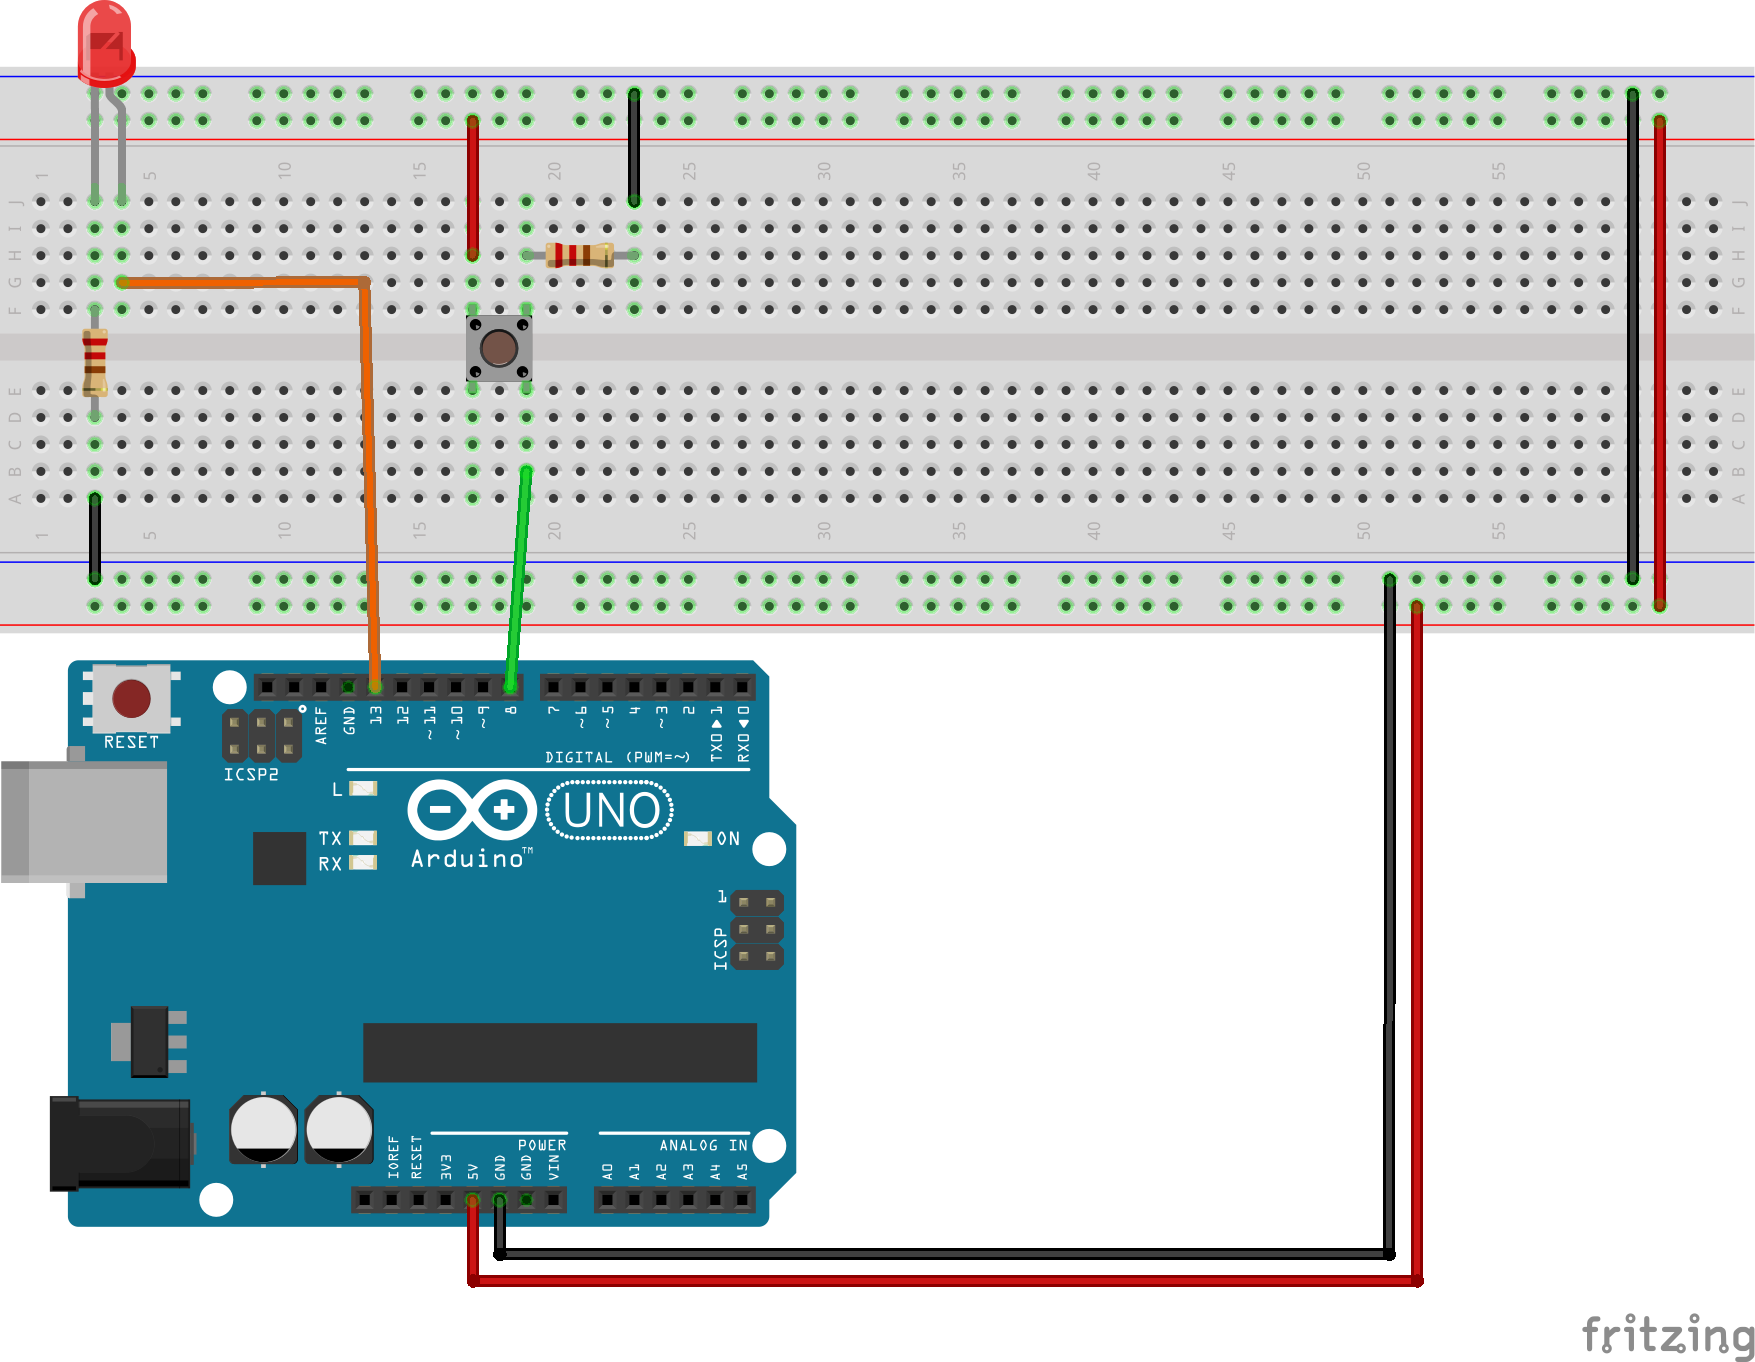
\includegraphics[height=6cm]{img/TP3-1.png}
	\caption{\label{TP3.1}LED et boutton}
\end{figure}


\subsection{Debounce}

\lstinputlisting[language=C]{Code/TP3/TP3.2/TP3.2.ino}
\begin{figure}[H]
	\centering
	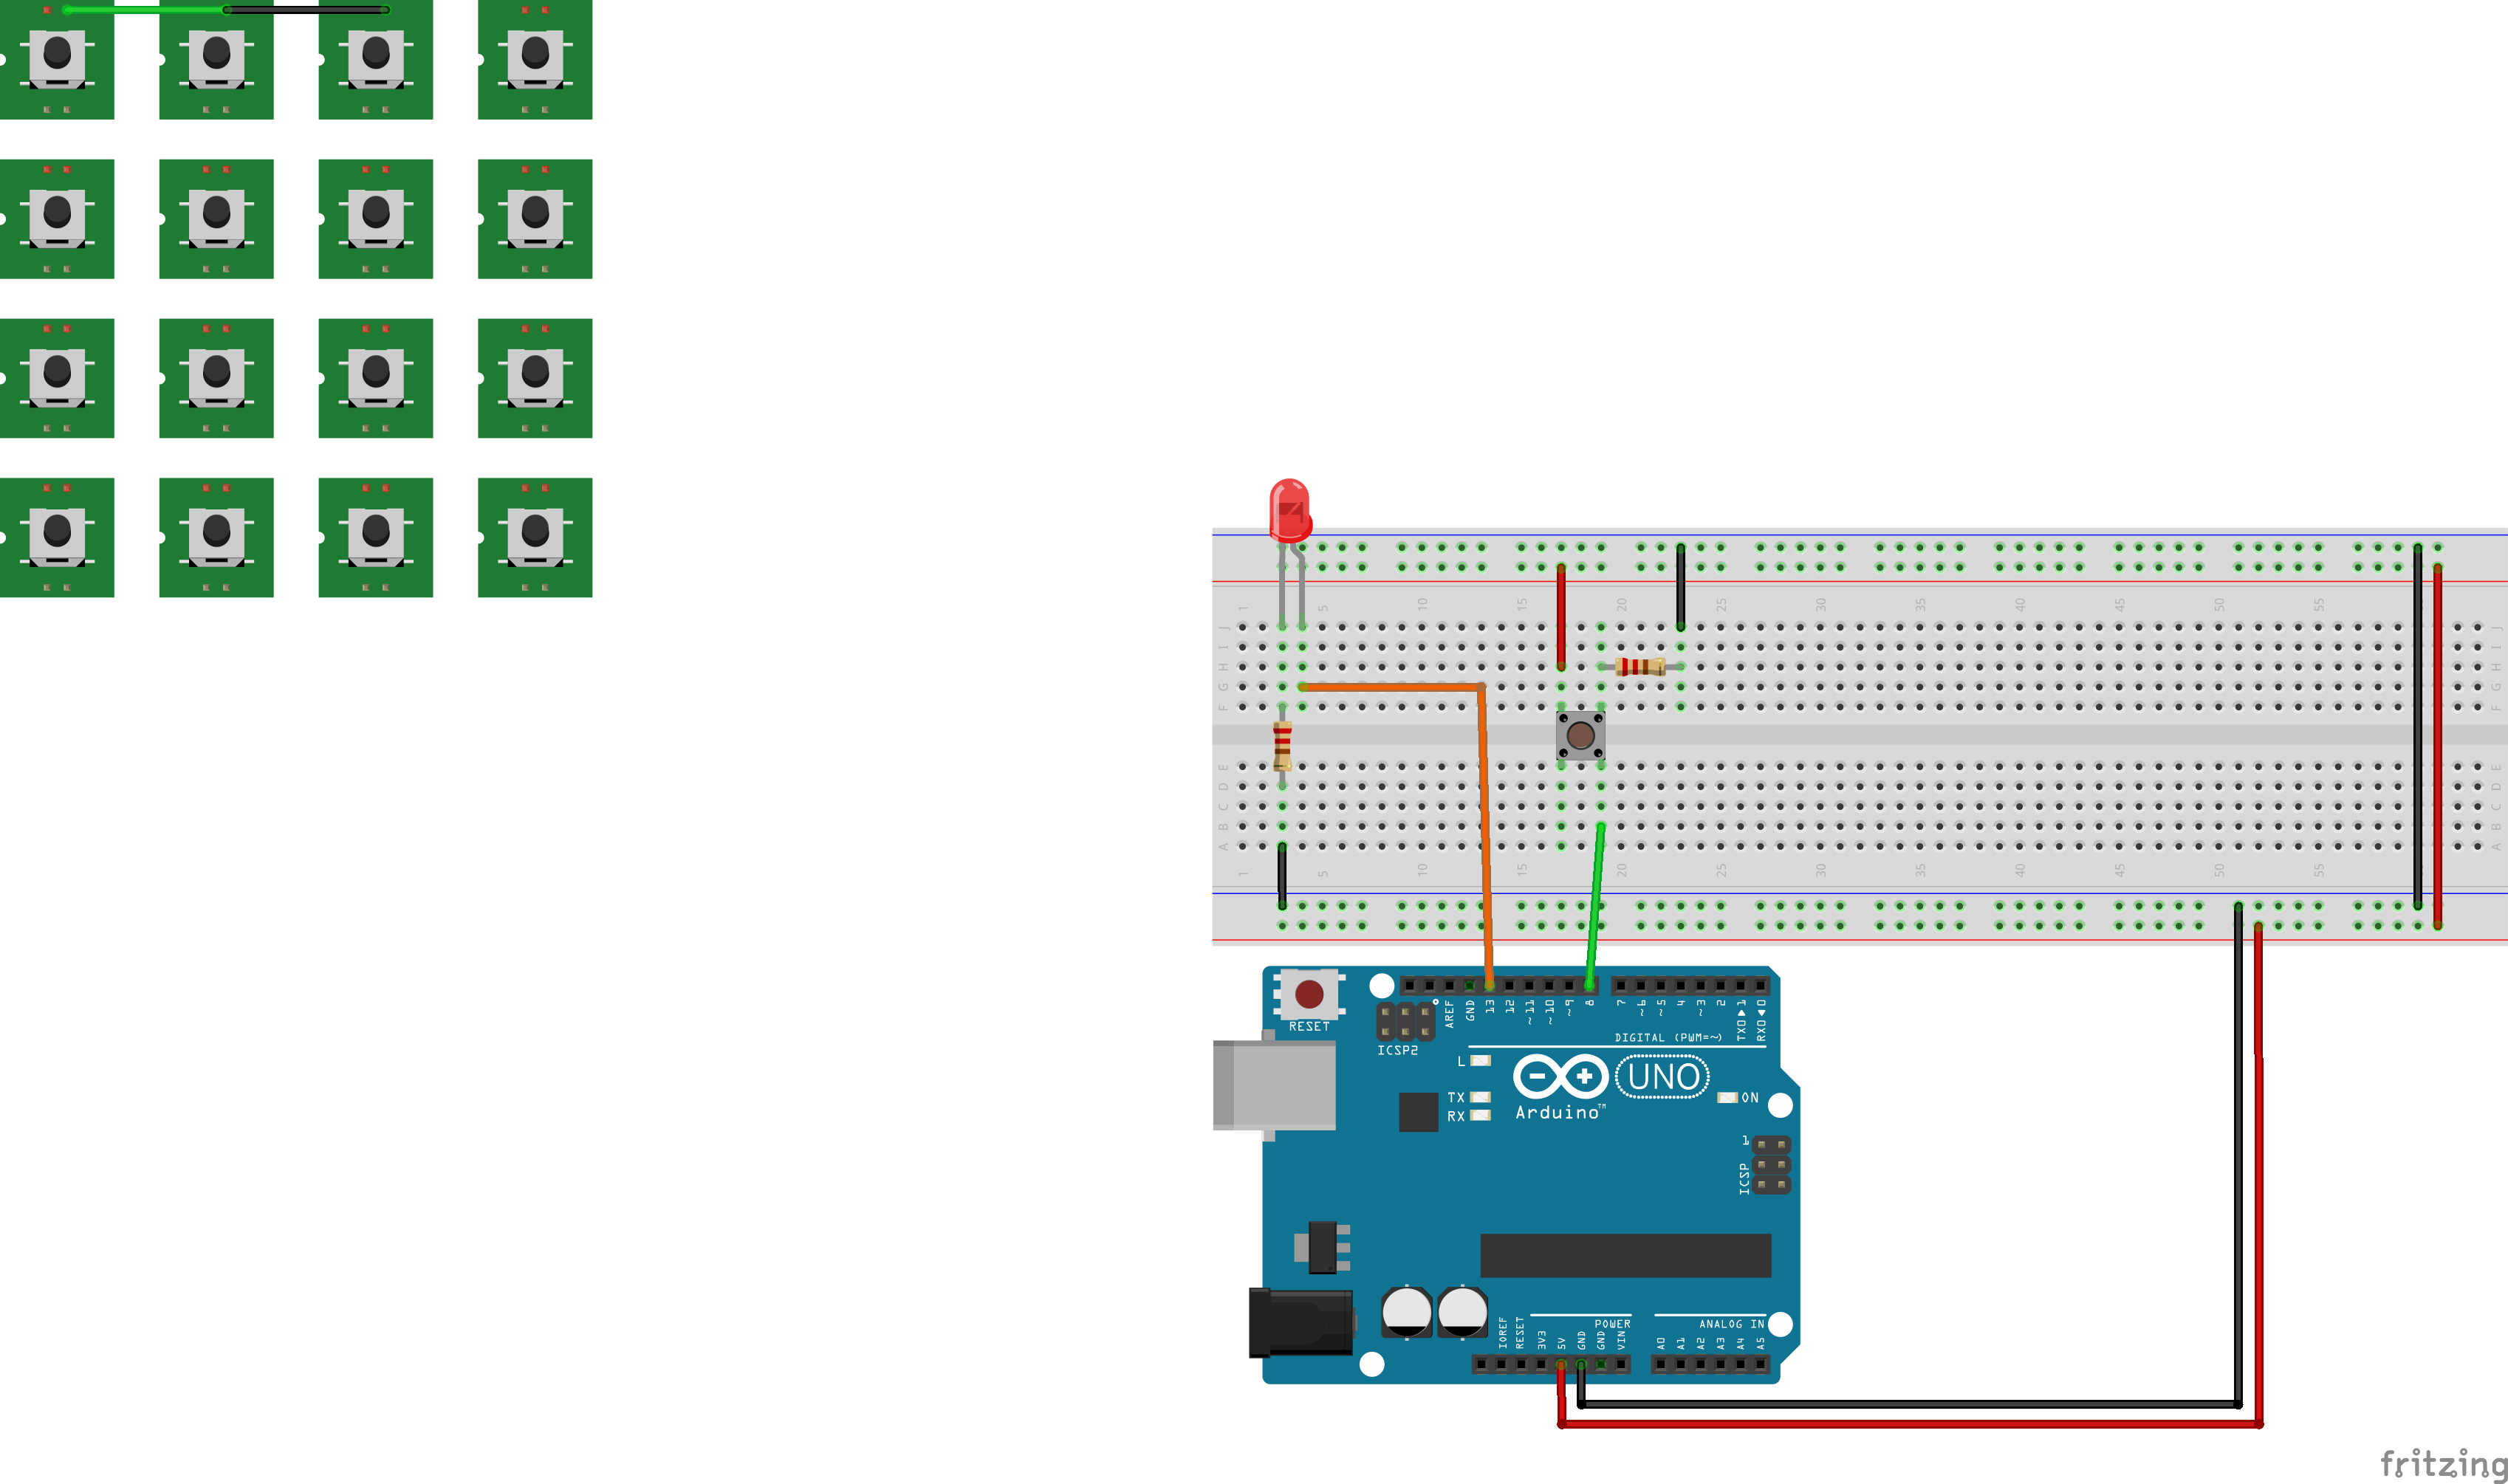
\includegraphics[height=6cm]{img/TP3-2.png}
	\caption{\label{TP3.2}Debounce}
\end{figure}

\subsection{Matrice de bouttons}

\lstinputlisting[language=C]{Code/TP3/TP3.3/TP3.3.ino}
\begin{figure}[H]
	\centering
	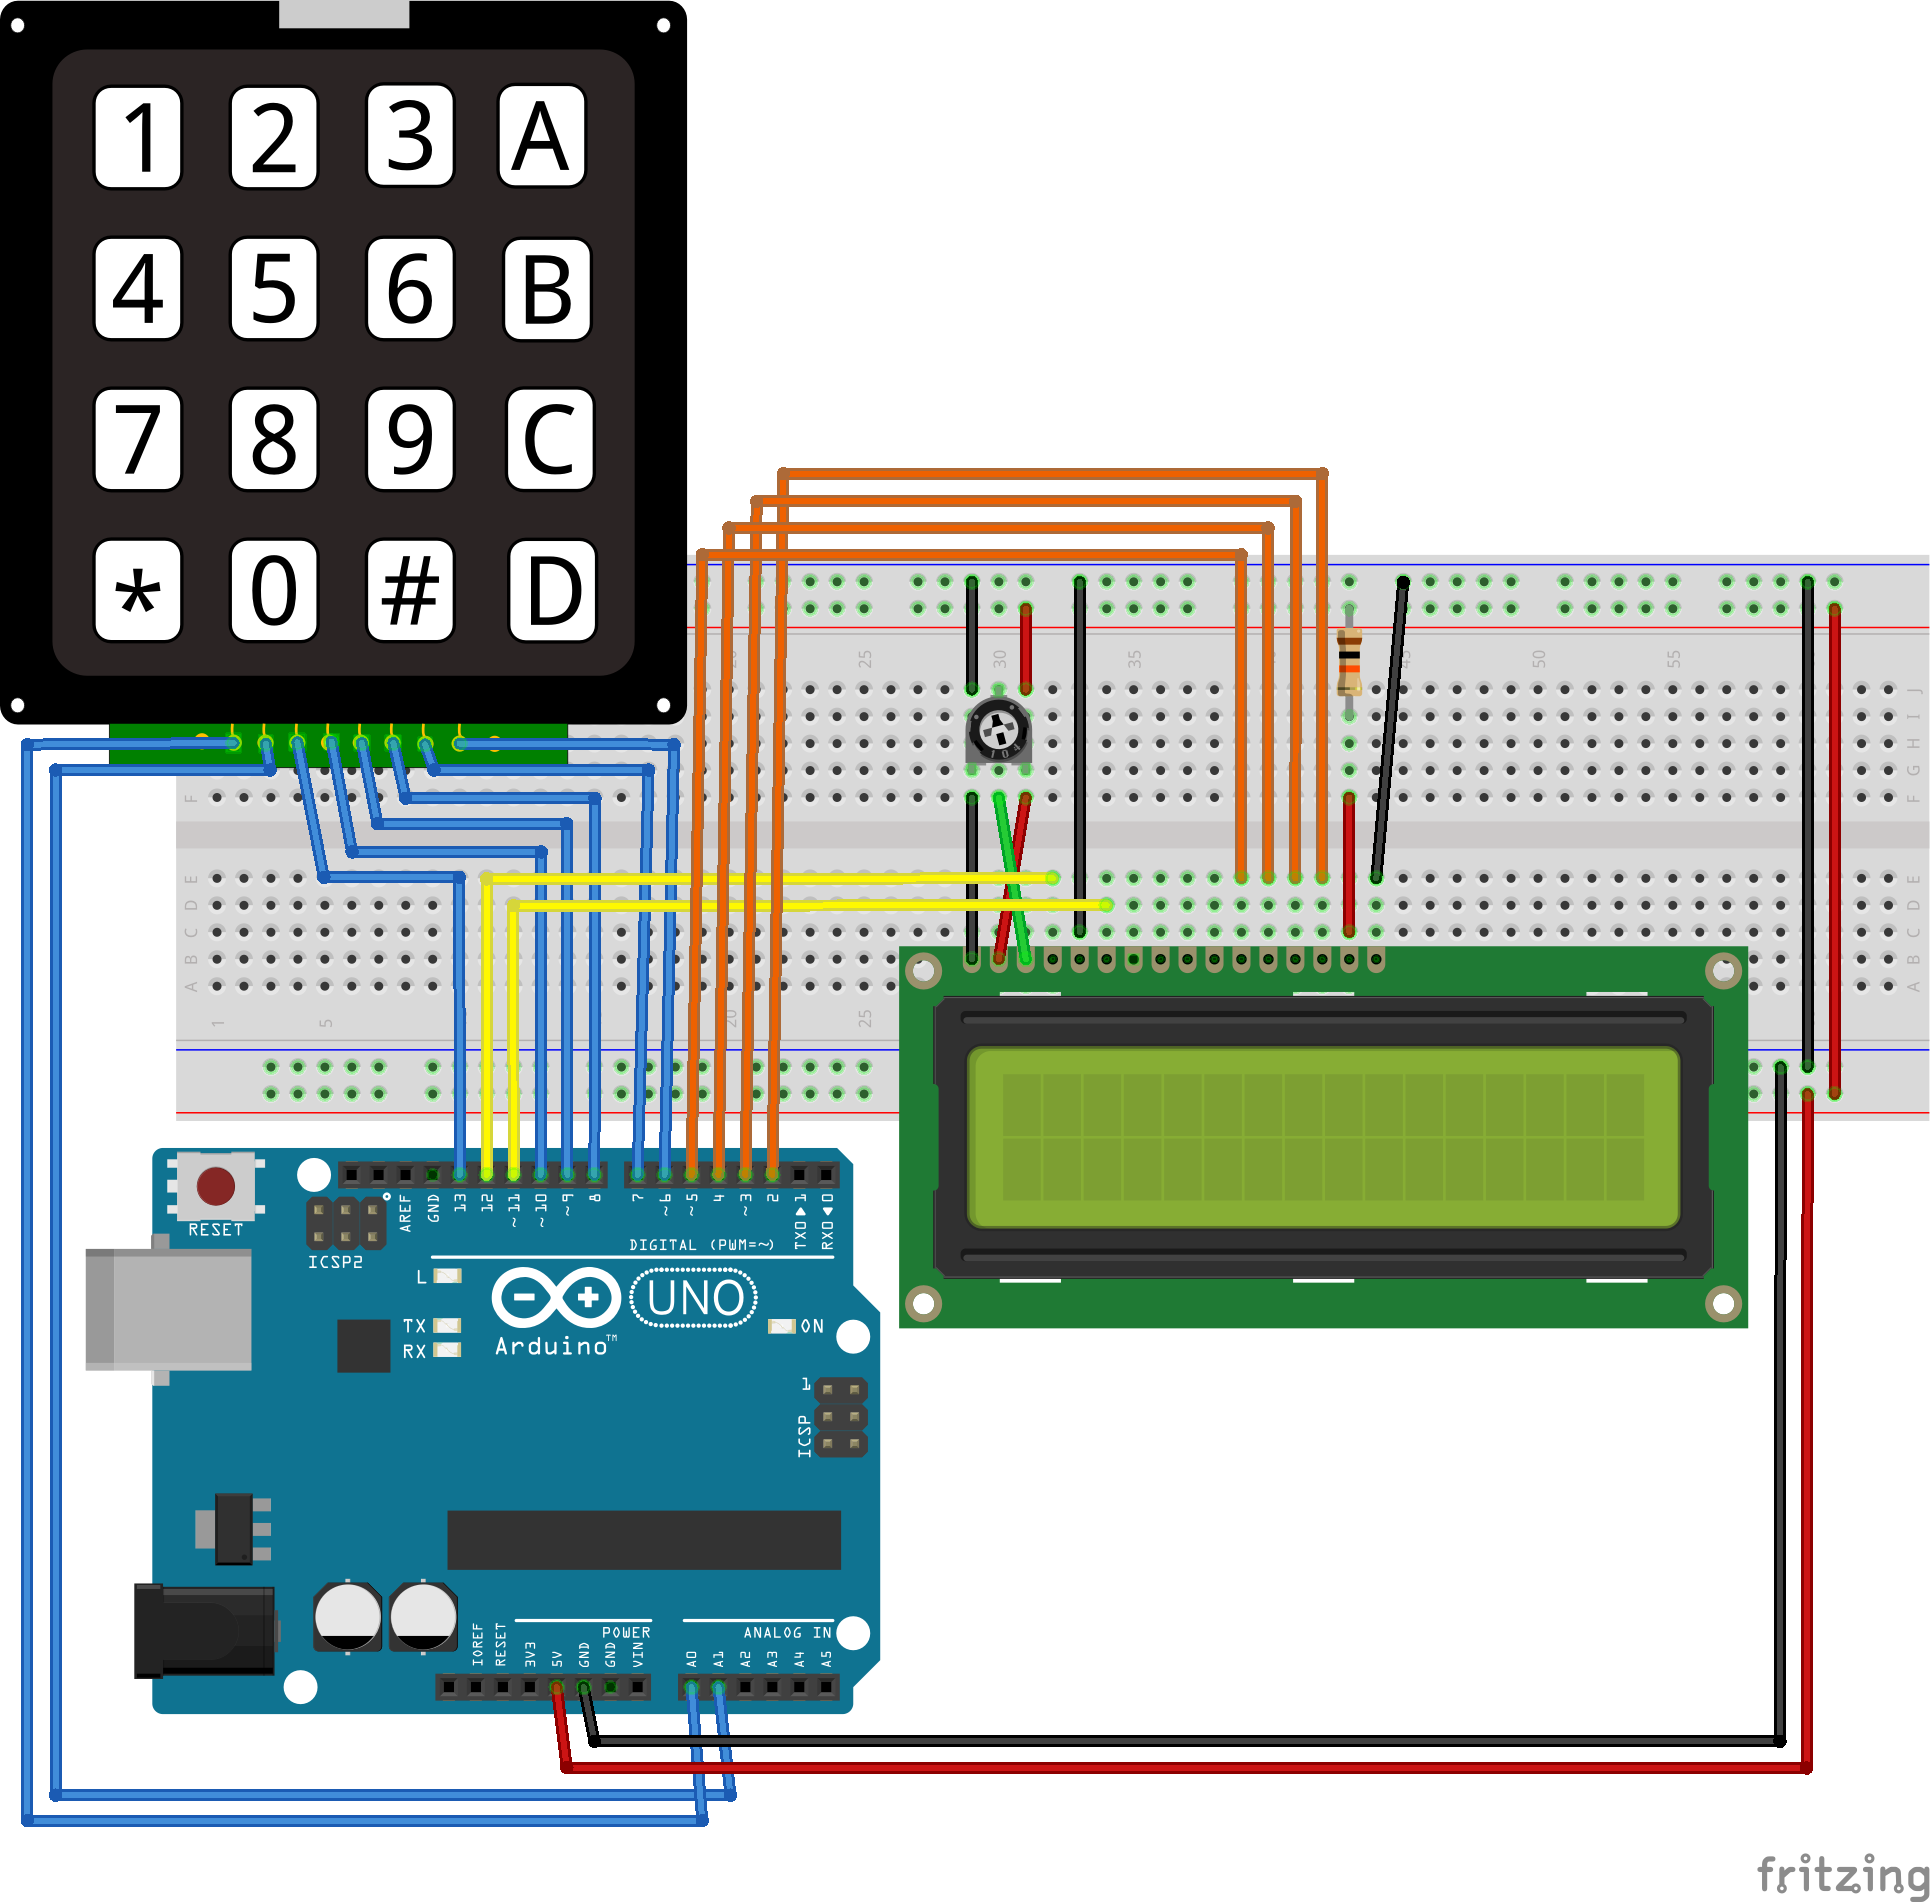
\includegraphics[height=6cm]{img/TP3-3.png}
	\caption{\label{TP3.3}Matrice de bouttons}
\end{figure}

% \subsection{Joystick et matrice de LED}

% \lstinputlisting[language=C]{Code/TP3/TP3.4/TP3.4.ino}
% \begin{figure}[H]
% 	\centering
% 	\includegraphics[height=6cm]{img/TP3-4.png}
% 	\caption{\label{TP3.4}Joystick et matrice de LED}
% \end{figure}

\clearpage
\section{Remerciement}
\label{sec:remerciement}

Je remercie Terencio \textsc{Agozzino} pour avoir réalisé la mise en page de ce document en \LaTeX.
\clearpage
\nocite{*}
\addcontentsline{toc}{section}{Références}
\bibliographystyle{acm} 
\bibliography{bibli}
\end{document}